% # 公立はこだて未来大学・修士論文テンプレートファイル(unicode)
%
% ## 改訂履歴:
% - 2019/12/01 初版 作成者:三上貞芳
% - 2020/01/12 V1.2 作成者:三上貞芳 英字綴訂正
%
% ## 論文作成の手順
%
% 1. 以下のtexファイルを作成してください
% - cover.tex           氏名・タイトル等の表紙情報
% - eabstract.tex       英語アブストラクト
% - jabstract.tex       日本語アブストラクト
% - chapterX.tex        本文第X章
% - publications.tex    発表・採録等の実績(確定分も含む)
% - acknowledgment.tex  謝辞
% - bibliography    .tex    参考文献
%
% 2. このテンプレートの「TODO: 本文」以下に,作成した章に対応する\input{chapterX.tex}文を追記してください(Xは章番号)
%
% 3. このテンプレートとfunstyle_master.texと合わせてuplatex環境でコンパイルし,PDFを作成します.
%

\documentclass[uplatex, a4paper, report, 11pt, oneside]{jsbook}

% packages
\usepackage[utf8]{inputenc}
\usepackage[dvipdfmx]{graphicx}
\usepackage{lmodern}             % use latin modern font
\usepackage{amsmath,amssymb,amsthm}
\usepackage{url}
\usepackage{here}

\usepackage{layout}

% 未来大書式設定
% % # 公立はこだて未来大学・修士論文書式定義ファイル
%
% (https://github.com/kmiya/naist-thesis-tmpl を一部参照)
% 
% ## 改訂履歴:
% - 2019/11/18 初版 作成者:三上貞芳

% ## 使用法;
% - main.texを参照してください.
% - **このファイルを変更する必要はありません**

\usepackage[dvipdfmx]{graphicx}
\usepackage[utf8]{inputenc}
\usepackage[T1]{fontenc}
\usepackage{lmodern}
\usepackage{amsmath,amssymb,amsthm}
\let\equation\gather
\let\endequation\endgather
\usepackage{fancybox}
\usepackage[flushmargin,symbol]{footmisc}
\usepackage[nottoc]{tocbibind}
\usepackage[dvipdfmx,%
 bookmarks=true,%
 bookmarksnumbered=true,%
 setpagesize=false,%
 colorlinks=false,%
 linkbordercolor={0.8 0.8 0.8},%
 citebordercolor={0.8 0.8 0.8},%
 pdfborder={0 0 0.6},%
% urlcolor=black,linkcolor=black,citecolor=black,%
 pdftitle={},% 修論のタイトルを入れる
 pdfauthor={},% 名前を入れる
 pdfsubject={Master's thesis},%
 pdfkeywords={\ekeywords}]{hyperref}
\usepackage{pxjahyper}

% ページレイアウト
\textheight=20.6truecm          % 縦
\textwidth=14.5truecm           % 横
\oddsidemargin=0.6truecm        % 左マージン(1inオフセット後)
\evensidemargin=-3.8truecm      % 右マージン(1inオフセット後)

% フォント等調整
% 参考文献
\def\thebibliography#1{\chapter*{参考文献\markboth
 {参 考 文 献}{参 考 文 献}\addcontentsline{toc}{chapter}{参考文献}}\list
 {[\arabic{enumi}]}{\settowidth\labelwidth{[#1]}\leftmargin\labelwidth
 \advance\leftmargin\labelsep
 \usecounter{enumi}}
 \def\newblock{\hskip .11trueem plus .33trueem minus -.07trueem}
 \sloppy
 \sfcode`\.=1000\relax}
\let\endthebibliography=\endlist

% 章
\makeatletter%%
\def\@makechapterhead#1{\hbox{}%
  \vskip-1\Cvs
  {\parindent\z@
%  \reset@font\LARGE\bfseries
   \raggedright\reset@font\Large\bfseries% 左揃え
   \ifnum \c@secnumdepth >\m@ne
     \setlength\@tempdima{\linewidth}%
     \vtop{\hsize\@tempdima%
         \@chapapp\thechapter\@chappos\mbox{\ \ }%
     #1}%
   \else
     #1\relax
   \fi}\nobreak\vskip1\Cvs}
\makeatother%%

\makeatletter%%
\def\@makeschapterhead#1{\hbox{}%
  \vskip-1\Cvs
  {\parindent \z@ \raggedright
    \normalfont
    \interlinepenalty\@M
    \Large\headfont #1\par\nobreak
    \vskip1\Cvs}}
\makeatother%%

% 節
\makeatletter%%
\renewcommand{\section}{%
  \@startsection{section}% #1 見出し
   {1}% #2 見出しのレベル
   {\z@}% #3 横組みの場合,見出し左の空き(インデント量)
   {1.5\Cvs \@plus.5\Cdp \@minus.2\Cdp}% #4 見出し上の空き
   {.5\Cvs \@plus.3\Cdp}% #5 見出し下の空き (負の値なら見出し後の空き)
  {\raggedright\reset@font\large\bfseries}% 左揃え
}%
\makeatother%%

% 小節
\makeatletter%%
\renewcommand{\subsection}{%
  \@startsection{subsection}% #1 見出し
   {1}% #2 見出しのレベル
   {\z@}% #3 横組みの場合,見出し左の空き(インデント量)
   {1.5\Cvs \@plus.5\Cdp \@minus.2\Cdp}% #4 見出し上の空き
   {.5\Cvs \@plus.3\Cdp}% #5 見出し下の空き (負の値なら見出し後の空き)
  {\raggedright\reset@font\normalsize\bfseries}% 左揃え
}%
\makeatother%%

% 表題
\makeatletter
\def\@startsection#1#2#3#4#5#6{%
  \if@noskipsec \leavevmode \fi
  \par
  \@tempskipa #4\relax
  \if@english \@afterindentfalse \else \@afterindenttrue \fi
  \ifdim \@tempskipa <\z@
    \@tempskipa -\@tempskipa \@afterindentfalse
  \fi
  \if@nobreak
    \everypar{}%
  \else
    \addpenalty\@secpenalty
    \ifdim \@tempskipa >\z@
      \vskip\@tempskipa
      \if@slide\else
        \null
        \vspace{-\baselineskip}%
      \fi
    \fi
  \fi
  \noindent
  \@ifstar
    {\@ssect{#3}{#4}{#5}{#6}}%
    {\@dblarg{\@sect{#1}{#2}{#3}{#4}{#5}{#6}}}}
\makeatother

% 式番号
\makeatletter
  \renewcommand{\theequation}{%
  \thesection.\arabic{equation}}
    \@addtoreset{equation}{section}
\makeatother


% 図番号
\makeatletter
 \renewcommand{\thefigure}{%
  \thechapter.\arabic{figure}}
   \@addtoreset{figure}{chapter}
 \makeatother
\makeatletter

% 目次に小節を表示
\setcounter{tocdepth}{4}


% TODO: タイトル・著者等の情報
% TODO: 論文題目等の情報を以下に記入

\newcommand{\jdoctitle}{修士論文}
\newcommand{\edoctitle}{Master's Thesis}
\newcommand{\jtitle}{人間とAIの協調:ChatGPTを用いたMinecraftBOTによる作業支援}  % 修論の題名
\newcommand{\etitle}{Human and AI Co-operation: Minecraft Server and Bots}   % 論文題目(英)
\newcommand{\jauthor}{工藤 光矢}      % 著者名(日)
\newcommand{\eauthor}{Koya Kudo} % 著者名(英)
\newcommand{\jadvisor}{フランク イアン}   % 指導教員名(日)
\newcommand{\eadvisor}{Ian Frank}  % 指導教員名(英)
\newcommand{\jdate}{2024年2月XX日}  % 論文提出日   (日)
\newcommand{\edate}{February XX, 2024}  % 論文提出年月 (英)
\newcommand{\jkeywords}{チャットボット,デジタルコラボレーション,空間創造性} % キーワード(日)
\newcommand{\ekeywords}{Chatbots, Digital Collaboration, Spatial Creativity}   % キーワード(英)
\newcommand{\eshorttitle}{Human and AI Co-operation: Minecraft Server and Bots}    % 短縮英題題名(おおよそ8 words以内)
\newcommand{\jaffiliation}{知能情報科学領域}    % 領域名(日)
\newcommand{\eaffiliation}{Intelligent Information Science Field}    % 領域名(英)


% TODO: 英語アブストラクト
% TODO: 英文アブストラクトを以下の{}内に記述(以下はダミーテキスト)
\newcommand{\eabstract}{

Games have long been important as a testbed and basic research for improving the performance of artificial intelligence and algorithms, and in recent years AI has surpassed human scores in complex games such as Go. 
However, even though AI has overwhelmed humans, game research is still valuable as a testbed and basic research, and new approaches, such as human-AI cooperation, are being seen. 
This research aims to explore the boundaries and possibilities of cooperation and collaboration between humans and AI in the context of ever-changing artificial intelligence technologies, and has developed a bot "Mason" (Minecraft AI Support - Objectives and Novelty) that works with players in the virtual 3D game "Minecraft" using the ChatGPT API. 
which can suggest the next task suitable for the current situation by observing the player's information and conversations with the player. 
It can also generate and customise structures such as houses and furniture in the gameplay world by issuing Minecraft fill commands according to user instructions. 
When these functions were tested, the LLM's spatial grasp and response performance suggested the boundaries of the current cooperation and collaboration between humans and AI. 
The ability to embed bot functions in virtual space is rapidly expanding, and these results can be seen as an early stage in the activity of embedding bots in virtual space. 
Minecraft also has applications as an educational tool, and Mason's potential for human-AI cooperation is that Mason can introduce students to the basics of virtual worlds Mason could be useful for introducing students to the basics of virtual worlds, developing their creativity and communication skills, and familiarising them with LLMs. 
Future plans include the need to improve the prompts to allow for more complex structures to be generated and interacted with, and for stronger inspiration and competence; the Mason framework is publicly available and could be adapted by others to explore the creative The possibility of exploring the perspectives enabled by the development of generative AI is also conceivable.

}

% TODO: 日本語アブストラクト
% TODO: 日本語アブストラクトを以下の{}内に記述(以下はダミーテキスト)
\newcommand{\jabstract}{

    ゲームは人工知能やアルゴリズムの性能向上のための実験台や基礎研究として古くから重要視されており,近年では囲碁などの複雑なゲームにおいてAIが人間のスコアを超越するようになった.
    しかし,AIが人間を圧倒してもなお,ゲーム研究は実験台や基礎研究として価値のあるものであり,人間とAIの協力関係と言った新たなアプローチが見られるようになっている.
    本研究では変化し続ける人工知能技術の中で,人間とAIとの協調・協力関係の境界と可能性を探ることを目的としており,仮想3Dゲーム「Minecraft」において,ChatGPT APIを活用してプレイヤーと連携するbot "Mason"(Minecraft AI Support - Objectives and Novelty)を作成した.
    Masonはプレイヤーとの会話やプレイヤーの情報を観察することで,現在の状況に適した次のタスクを提案することができる.また,ユーザーの指示に従ってMinecraftのfillコマンドを発行することで,ゲームプレイの世界に家や家具などの構造物を生成し,カスタマイズすることもできる.これらの機能をテストしたところ,LLMの空間把握能力や応答性能から,現状の人間とAIとの協調・協力関係の境界が示唆された.ボット機能を仮想空間に埋め込む能力は急速に拡大しており,この結果はbotを仮想空間に埋め込む活動の初期段階とみなすことが出来る.Minecraftは教育ツールとしての用途もあり,Masonの人間とAIの協調の可能性として,Masonは生徒に仮想世界の基礎を紹介したり,創造性やコミュニケーション力を鍛え,LLMに慣れ親しんでもらうのに役立つと考えられる.今後の予定としては,プロンプトの改善によってより複雑な構造物を生成や対話を可能にし,より強いインスピレーションや能力を得られるようにする必要があると考えられる.Masonフレームワークは公開しており,他の人が適応して,生成AIの発展によって可能になった創造的な展望を探求可能性も考えられる.

}

% page size
\textheight     = 22.6truecm
\textwidth      = 14.7truecm
\oddsidemargin  = 0.6truecm

% header and footer
\usepackage{fancyhdr}
\pagestyle{fancy}
\setlength{\footskip}{16pt}
\fancyhf{}
\renewcommand{\chaptermark}[1]{\markboth{\thechapter.\ #1}{}}
\rhead{\leftmark}
\renewcommand{\headrulewidth}{0pt}
\cfoot{\thepage}
\lfoot{~~ \\Master's thesis, Future University Hakodate}
\lhead{\eshorttitle}

%-------------------------------------
\begin{document}

\thispagestyle{empty}
\vspace*{1.5truemm}
\begin{center}
    \LARGE\bfseries
    修士論文
\end{center}
\vspace*{2truemm}
\begin{center}
    \LARGE\bfseries\jtitle
\end{center}
\vspace*{2em}
\begin{center}
    \large\bfseries 公立はこだて未来大学大学院~~システム情報科学研究科\par%
    \jaffiliation
\end{center}
\vspace*{1em}
\begin{center}
    \Large\bfseries\jauthor
\end{center}
\vspace*{1em}
\begin{center}
    \large 指導教員~~~~\jadvisor\par
    \vspace{0.5em}
    \large 提出日~~~~\jdate
\end{center}
\vspace*{3em}
\begin{center}
\textbf{\Large Master's Thesis}\par
\vspace*{2em}
\textbf{\Large \etitle}\par
\vspace*{1em}
{\normalsize by}\par
\vspace*{1em}
{\large \eauthor}\par
\vspace*{1.5em}
Graduate School of Systems Information Science, Future University Hakodate \par
\eaffiliation

% \vspace*{0.5em}
\normalsize Supervisor: \quad \eadvisor \par
\vspace*{2em}
Submitted on \edate
\end{center}
%\vspace*{\fill}

% 英語アブストラクト作成
\newpage
\thispagestyle{empty}
\vspace*{30truemm}
\noindent
\textbf{Abstract--}~
\eabstract

\vspace*{1em}
\noindent
\textbf{Keywords:}~ 
\ekeywords

% 日本語アブストラクト作成
\newpage
\thispagestyle{empty}
\vspace*{30truemm}
\noindent
\textgt{概~要:}~
\jabstract

\vspace*{1em}
\noindent
\textgt{キーワード:}~ 
\jkeywords


% 目次
\tableofcontents
\thispagestyle{empty}

% ページ番号初期化
\setcounter{page}{0}

% TODO: 本文
\chapter{序論}	
\thispagestyle{plain}   % chapterの直後に必ず指定

本章では``人間とAIの協調:ChatGPT を用いたMinecraftBOT による作業支援''の研究を行うに至った背景や目的,また本稿の章構成を述べる.

\section{背景・目的}
本研究では変化し続ける人工知能技術の中で,人間とAIとの協調・協力関係の境界と可能性を探ることを目的としている.
目的の達成のために,Minecraft内での人間との対話や作業支援を行うbotの開発を通じて検証を行った.

本研究の背景としては,``チェスはAIのショウジョウバエである''\cite{bib:chess}と言うように,ゲームは人工知能やアルゴリズムの性能向上のための実験台や基礎研究として古くから重要視されてきたことがあげられる.
特に2010年代に入ってからは,囲碁やスタークラフトといった複雑なゲームにおいて,AIが人間のスコアを超越するようになった\cite{bib:AplpaGo,bibAlphaStar}.
しかし,AIが人間を圧倒してもなお,ゲーム研究は実験台や基礎研究として価値のあるものであり,ここ数年では,人間とAIの協力関係と言った新たなアプローチが見られるようになっている\cite{bib:maia,bib:craft_assist}.
さらに2023年からは,ChatGPT\cite{bib:chatgpt}の登場により大規模言語モデルの利用が大きく広がり,ChatGPTは2ヶ月で利用者が1億人を突破した\cite{bib:chatgpt_news}.ま
た,大規模言語モデルを使用したテキストベースで対話可能なサービスが登場している\cite{bib:citegpt, bib:slidegpt}.

一般的にAIの研究で使用されるゲーム環境として,``Minecraft\cite{bib:Minecraft}''が使用されている.
Minecraftは2014年に最も売れたインディーゲームとして,2023年には3億本を売り上げた認知度の高いゲームである\cite{bib:minecraft_news}.
また,Minecraftは,ユーザーが自由に世界を創造・探索できるゲームであり,その特性から教育や研究のツールとしても幅広く使われている.

そこで本研究では,Minecraftのその特性に焦点を当て,Minecraftの中で大規模言語モデルを搭載したbot,{\mason} (Minecraft AI Support - Objectives and Novelty)を作成した.{\mason}と人間が対話を行ったり,共同作業を行ったりすることで,人間とAIの協力・協調関係の検証を行う.
bot機能を仮想空間に埋め込む能力は急速に拡大しており,対話型インターフェースの進化が検証されている.本研究はbot機能を仮想空間に埋め込むこれらの研究と同様の,初期の研究とみなすことができる.
botの行った建築作業などからは,人間が建築する際の新たなアイデアやインスピレーションを得られる可能性があると考える.

\section{章構成}
本稿の章構成について解説する.
第2章では本研究に関する,人間とAIの協調,Minecraftの教育性,自動生成,Minecraftのエージェント等の研究,文献について述べる.
第3章では本研究のゲーム環境であるMinecraftやテスト環境のFUN Minecraft Serverについて述べる.
第4章では本章では作成したbot,{\mason}についてや,各節で{\mason}の詳細な機能について解説する.
第5章ではMasonの動作テストや構造物自動生成の実験,アンケート実施等の概要や結果について述べる.
第6章では本研究の考察について述べる.
第7章では本研究のまとめや展望について述べる.
\chapter{関連研究}	% TODO: 章題を記入.題は任意.
\thispagestyle{plain}   % chapterの直後に必ず指定

%TODO: 章の内容を記入.以下はサンプル.

\section{〇〇の研究}
この節では人間との協調を目的としたAIに関する関連研究について述べる.

\subsection{Maia}
Kleinbergらは,人間らしい手を打つニューラルネットワークチェスエンジンの“Maia”を開発した.
Maiaはオンラインでチェスを行うプレイヤーの棋譜を,強さ別に9つのレベルに分けて学習しており,レベル別にプレイヤーがどのようなチェスの指し方をしているかを学べるようになったと述べている.
また,低いレベルと高いレベルの学習結果の違いから,未熟なチェスプレイヤーがどのような間違いを犯すかを「チェス学習ツール」として予測することが出来る.
Kleinbergは,人間に教えたり助けたりするAIの研究によって,人間ともっとうまく交流できるかもしれない,あるいは交渉すらできるかもしれないと述べている.

\subsection{学習ツールとしてのMinecraft}
Cipolloneらは高校の文学の授業でMinecraftを使用し,文学の授業を受けた生徒らはMinecraftを録画する形で映画を3本作成した.
Cipolloneらは作成された映画をプロットとキャラクターの観点で検討したところ,Minecraftを用いたことで生徒が創造性を発揮し,概念を理解しやすくなったと述べている.
また,Minecraftは他の方法ではコストがかかったり不可能だったりするような作品を生徒が作れるようになるツールであると述べている.
しかし,ゲーム文化と,正式な学校教育の文化とではギャップが大きいため,Minecraftのような教育ゲームを導入するためには,ゲーム文化をもっと受け入れられるような考えが必要かもしれないと提案している.

\subsection{ARLPCG}
Gisslénらは,手続き型コンテンツ生成の新たなアプローチとして,Adversarial Reinforcement Learning for Procedural Content Generation(ARLPCG)を提案した.
手続き型コンテンツ生成の一般的なアプローチとしては,異なる環境を手続き的に生成し,学習したエージェントの汎用性を高める方法が挙げられるが,ARLPCGでは代わりに,PCGエージェント(Generator)と攻略エージェント(Solver)からなる敵対的モデルを用いている.
GeneratorはSolverのパフォーマンスに基づいて報酬信号を受け取っており,攻略不可能ではないが挑戦的なコンテンツ生成が可能になったと述べている.
また,モデルの制御を行うためにGeneratorに補助入力を使用し,検証として3DCGのアクションゲームとレースゲームの2つを生成したところ,ARLPCGの解答率が大幅に向上し,補助入力によって難易度がある程度調整可能になったと述べている.

\subsection{GANcraft}\label{sec:gancraft}
Haoらは、Minecraftのような3Dのブロック世界からリアルな地形画像を生成する、GANcraftを開発した。
GANcraftは教師なしのニューラルレンダリングフレームワークである。
本手法では、ブロック世界を入力とし、各ブロックには土、草、木、砂、水などのラベルが割り当てられる。
また、ブロックの世界を連続的な体積関数として表現し,教師データがない場合でも,任意の視点からなリアルな地形画像をレンダリングできるようにモデルを学習できると述べている。
GANcraftは、その他のフレームワークと比較して有効性を示しており、長年の経験が必要とされる複雑な風景の3Dモデリングを簡単に行うことができると述べている。

\subsection{CraftAssist}
Grayらは、Minecraftで人間のプレイヤーと協力できるAIアシスタントを実装するためのプラットフォームとして、CraftAssistを開発した。
CraftAssistのアシスタントはブロックの配置や破壊、人間のプレイヤーとのチャットが可能であり、また、言語、知覚、記憶、身体的動作を組み合わせることで、家の建設などの複雑なタスクを実行できる。
このような研究は、実世界で人間とより良く対話し協力できるAIアシスタントを実現する手助けとなる可能性があり、AIアシスタントとの対話を通じて新しい概念とスキルを積極的に学び取ることができるかもしれないと述べている。

\subsection{Voyager}
Wangらは、MinecraftでLLMを使用し、人間の介入なしに継続的に世界を探索するエージェントのVoyagerを開発した。
VoyagerはAPIを介して自分の所持アイテムや近くの地形などのゲーム情報を読み取ることができ、GPT-4を用いて、情報をもとに短期的な目標を設定したり、目標を達成するために必要なコードを生成したりすることが可能である。
Voyagerはほかのモデルと比較して広い範囲の地形を探索し、多くのアイテムを製作することができたと述べている。
またWIRED誌では``このような方法で言語モデルを活用すれば、オフィスで多くの日常的な作業を自動化できるかもしれない。それがVoyagerがもたらした最大の経済効果であろう''と述べられている。

\chapter{Minecraftとは}	% TODO: 章題を記入.題は任意.
\thispagestyle{plain}   % chapterの直後に必ず指定

%TODO: 章の内容を記入.以下はサンプル.

\chapter{開発} 
\thispagestyle{plain}   % chapterの直後に必ず指定

本研究は,\ref{sec:minecraft}章で述べたMinecraftの特性に焦点を当て,Minecraftの中で大規模言語モデルを搭載したbotを作成し,そのbotと人間が対話を行ったり,共同作業を行ったりすることで,人間とAIの協力・協調関係の境界と可能性を探求することを目的としている.

本章では作成したbot、``Mason''について解説する.
システムの全体像は図\ref{fig:system}のとおりである.
プレイヤーはbotログイン用webアプリケーションを使用して,MasonをMinecraftのマルチサーバーに参加させることが可能である.
その後プレイヤーは,Masonが参加したマルチサーバーと同じサーバーにログインしMinecraftのチャットの機能(デフォルトでTキー)を用いてMasonと対話することが可能である.

MasonはMineflayer API\cite{bib:Mineflayer}を利用して実装されている.
Mineflayerは,botのセットアップやプレイヤーの発話や情報,ワールドの情報を読み取る機能、Minecraft内での行動を起こす機能などを総合的に提供するAPIである.
プレイヤーからの発話や情報はモードに合わせて、適切な大規模言語モデルに送り,大規模言語モデルからの返答をもとにプレイヤーへ返答や行動を行うことが可能である.

詳細な機能については\ref{sec:webapp}節から\ref{sec:build_mode}節で解説する.

\begin{figure}[H]
    \centering
    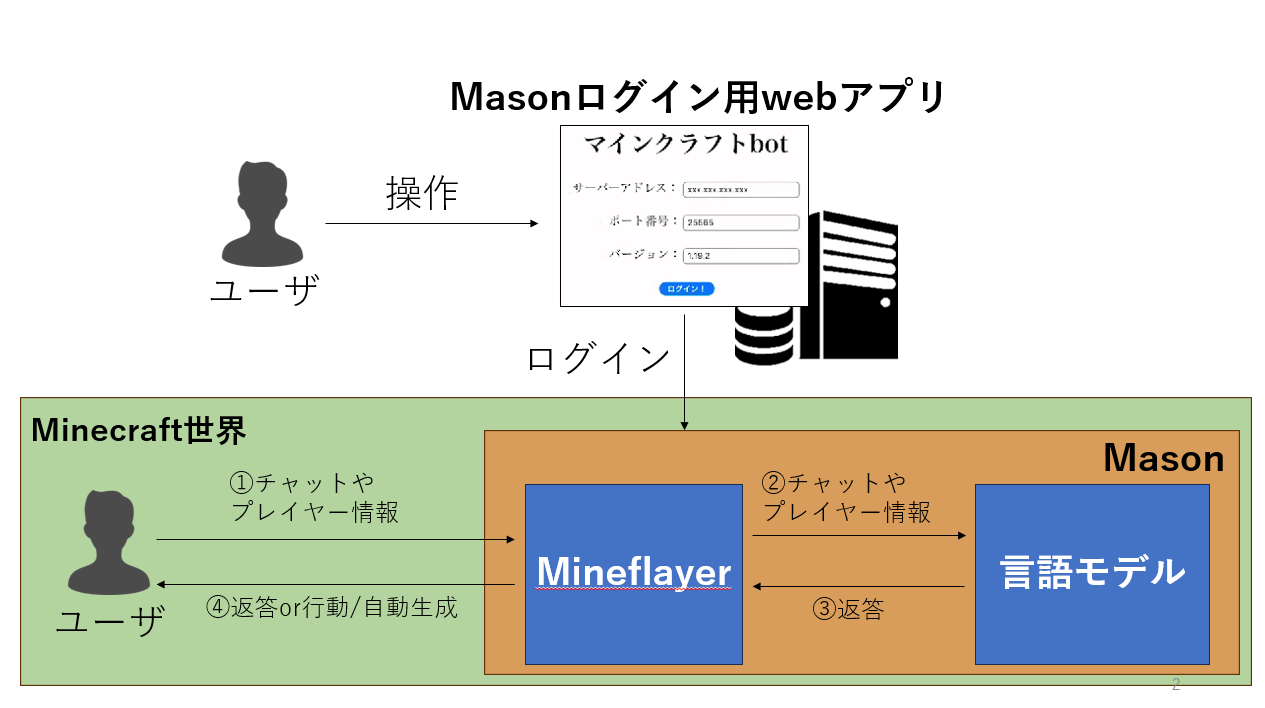
\includegraphics[width=0.7\textwidth]{fig/my_system.PNG}
    \caption{システムの概要}
    \label{fig:system}
\end{figure}

\section{Webアプリケーション}\label{sec:webapp}
人間とAIの協力・協調を主目的とする以上,ユーザビリティについて追求する必要があると考えたため,botをログインさせるためのWebアプリケーションを作成した.
従来までの方法でbotを動かすためには,プログラミング環境構築のスキルを必要とするが,このアプリケーションではマイクラのマルチにログインする時と同様の情報を入力することで,簡単にbotをログインさせることが可能となった.

\begin{figure}[H]
    \centering
    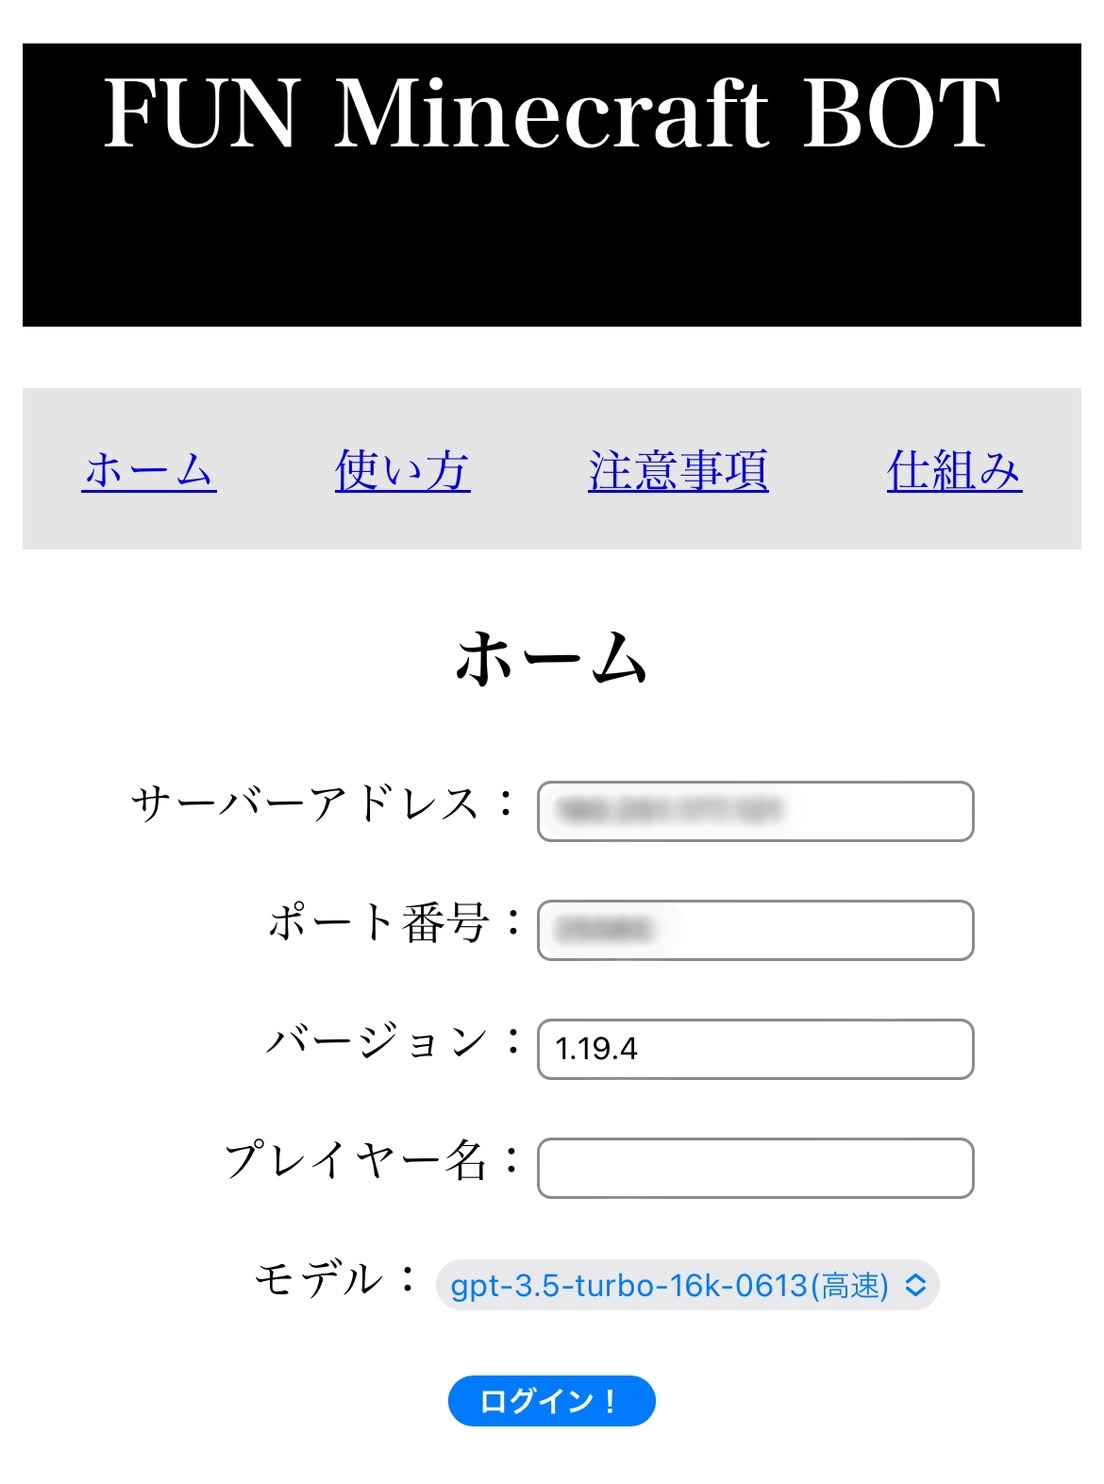
\includegraphics[width=0.5\textwidth]{fig/web_app.jpg}
    \caption{Webアプリケーションのホーム画像}
    \label{fig:web_app}
\end{figure}

\section{行動}\label{sec:act}
MasonがMinecraft世界に干渉して人間の作業などを手伝うことができるように,いくつかの行動を作成した.
Masonの各行動はMineflayer API\cite{bib:Mineflayer}を用いて実装した.
Mineflayer APIの関数は例外が発生するとbotがログアウトしてしまうため,基本的にMineflayer APIの関数に例外処理を加えて開発している.
作成した行動には表\ref{tab:action}の種類がある.

\begin{table}[H]
    \caption{行動の種類}\label{tab:action}
    \centering
    \begin{tabular}{lp{0.7\linewidth}}
        \hline \hline
        move\_to\_position & 説明: 指定した座標へ移動. \\
          & 引数: int x, int y, int z \\
        \hline
        mine\_block & 説明: nameで指定したブロックを指定個数採掘して集める. \\
          & 引数: str name, int count \\
        \hline
        smelt\_item & 説明: item\_nameで指定したアイテムをcountの個数分かまどで製錬する.fuel\_nameで燃料を指定する. \\
          & 引数: str item\_name, str fuel\_name, int count \\
        \hline
        mine\_block & 説明: nameで指定したブロックを指定個数採掘して集める \\
          & 引数: str name, int count \\
        \hline
        craft\_item & 説明: nameで指定したアイテムをcountの個数分,作業台で作成する. \\
          & 引数: str name, int count \\
        \hline
        get\_item\_chest & 説明: chest\_positionで指定した位置にあるチェストから,item\_dictのアイテムを個数分取り出す. \\
          & 引数: Vec3 chest\_position, dict[str,int] item\_dict \\
        \hline
        deposit\_item\_chest & 説明: chest\_positionで指定した位置にあるチェストに,item\_dictのアイテムを個数分入れる. \\
          & 引数: Vec3 chest\_position, dict[str,int] item\_dict \\
        \hline
        check\_item\_chest & 説明: chest\_positionで指定した位置にあるチェストのアイテムを確認する. \\
          & 引数: Vec3 chest\_position \\
        \hline
        farm & 説明: 近くの農地に所持している小麦の種を植える. \\
          & 引数: なし \\
        \hline
    \end{tabular}
\end{table}

\section{大規模言語モデルによるタスクの提示や会話}\label{sec:gpt_res}
複数の大規模言語モデルを組み合わせることによって,サバイバルモードのプレイヤー向けの対話機能を作成した.
この機能では,プレイヤーの発話と情報を元に,Masonが次のタスクを提示したり,\ref{sec:act}節の行動を起こすことでプレイヤーの作業を手伝ったり,質問や会話に返答することが可能になった.

プレイヤーの発話とは「how to make \textasciitilde?」,「please craft \textasciitilde.」,「please tell me next task.」のような,Masonに対する会話である.

プレイヤーの情報とは表\ref{tab:player_data}に示す,プレイヤーの現在の状態を表したJSONデータである.
\begin{table}[H]
    \caption{行動の種類}\label{tab:player_data}
    \centering
    \begin{tabular}{llp{0.6\linewidth}}
        \hline \hline
        キー & データ型 & 説明 \\
        \hline
        goals & string & プレイヤーの目標. \\
        biome & string & プレイヤーが現在居るバイオーム. \\
        time & string & Minecraft世界の現在時刻.0~23999までの値であり,13000~は夜を表す. \\
        blocks & list[string] & プレイヤーの半径10ブロック以内のブロックの種類 \\
        entities & list[string] & プレイヤーの半径10ブロック以内のエンティティの種類 \\
        health & string & プレイヤーの体力(20が最大) \\
        hunger & string & プレイヤーの満腹度(20が最大) \\
        pos & string & プレイヤーの現在の3次元座標 \\
        equip & list[string] & プレイヤーの装備中のアイテム(右手,左手,頭,体,脚,足) \\
        collected & list[string] & プレイヤーがこれまでに集めたアイテム \\
        chest & list[string] & 近くのチェスト \\
        \hline
    \end{tabular}
\end{table}

サバイバルモードのプレイヤー向けの対話機能の全体像や,プレイヤーの発話や情報の処理手順を図\ref{fig:interactive_function}に示す.
処理の手順としてまず,Chat Classificationモデルがプレイヤーの発話と情報を受け入れ,few-shot学習\cite{bib:few-shot}を使用してプレイヤーの発話を``Chat'',``Order'',``Request Next Task''の3つのカテゴリのいずれかに分類する.

発話が``Chat''に分類された場合,Chatモデルを用いて一般的な会話や質問に対応することができる.
このモデルはRetrieval-Augmented Generation (RAG)\cite{bib:rag}を用いており,通常は応答することが不可能な情報に対しても,大量のデータを参考にして応答を生成することが可能である.
RAGを用いる例として,Masonのテスト環境である,FUN Minecraft Server\cite{bib:fun_minecraft_server}に関する質問などが挙げられる.
これらの情報はインターネット上に情報が少ないことからもとのGPTモデルが学習しておらず回答が不安定であるが,RAGによってMasonはそれらの特定の条件に関する質問に答えることが出来る.

発話が``Order''に分類された場合,Actionモデルを用いてMasonが命令を解釈した後,表\ref{tab:action}の行動を実行し,プレイヤーの作業を手伝うことが可能である.
Orderに分類されるプレイヤーの発話の例としては,``cut the tree''などのMasonに対する命令文が考えられる.
命令文を受け取ると,Actionモデルでは,OpenAIのfunction calling\cite{bib:function_calling}によって適切な関数と引数が設定され,mine\_block("oak\_log",3)のように行動を実行することが可能である.

``Request Next Task''の分類では,プレイヤーの発話や情報がNext Taskモデルに,受け渡される.
Next TaskモデルのプロンプトはVoyager\cite{bib:voyager}のプロンプトに基づいており,プレイヤーの発話と情報から,Masonがプレイヤーに対して次のタスクを提示する.
また,提案されたタスクはActionモデルに渡され,Actionモデルが行動を実行できる場合は,プレイヤーのタスクを支援することができる.
例えば,プレイヤー情報のcollectedのリストが空である場合,モデルはプレイヤーがまだアイテムを集めたことがなく初期状態であると推論し,Minecraftにおける最初のタスク``cut the tree''などをプレイヤーに提案する.
そして提示した``cut the tree''というタスクはActionモデルにわたり,mine\_block("oak\_log",3)といった行動を起こすことが出来る.
したがって,Masonは初期状態のプレイヤーに対して``cut the tree''というタスクを提示し,同時にMasonも木を切って作業を手伝うことが出来る.

\begin{figure}[H]
    \centering
    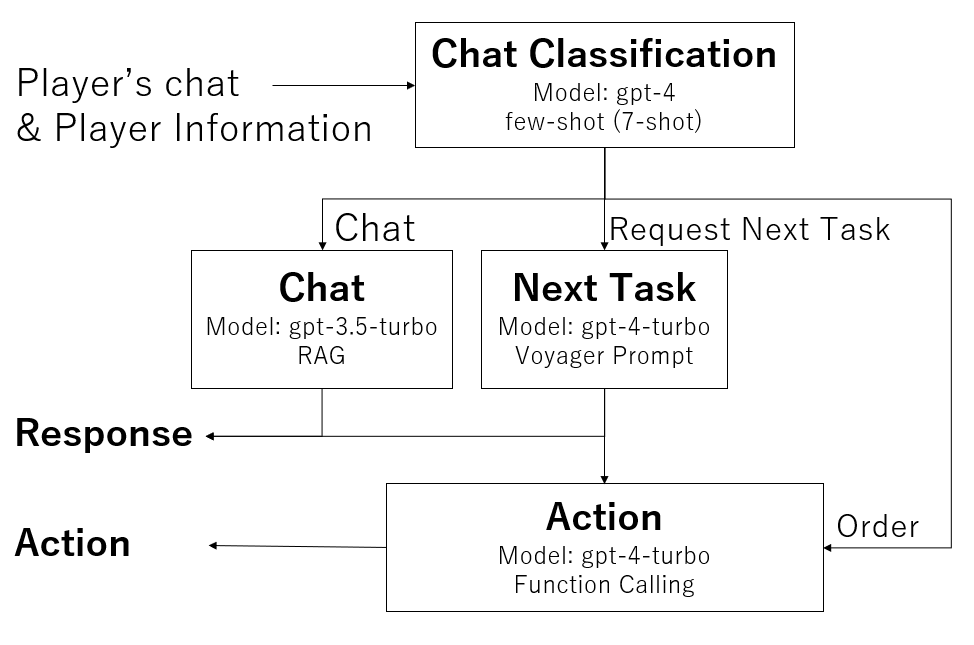
\includegraphics[width=0.8\textwidth]{fig/interactive_function.PNG}
    \caption{サバイバルモード向け対話機能の全体像}
    \label{fig:interactive_function}
\end{figure}

\section{構造物自動生成}\label{sec:build_mode}
独自のプロンプトによって,クリエイティブモードのプレイヤー向けに構造物の自動生成が可能になった.
このプロンプトには,/fillコマンドで構造物を生成すること,/fillコマンドの説明,3次元座標の概念の説明,/fillコマンドの使用例を記述した.

このプロンプトを初期プロンプトとして,作りたい構造物のプロンプトを送ると,fillコマンドのリストが提示され,fillコマンドのリストをMineflayerを通して順番に実行すると構造物が生成される.
また,追加のプロンプトを使用して装飾を追加したり,修正を加えたりすることができる.

この機能によって自動生成できる構造物の一例を図\ref{fig:generate_example}に示す。生成できる構造物については\ref{sec:build_mode_generate}節でその他多くの例を示し、その結果の考察について\ref{sec:generate_investigation}で述べる.

\begin{figure}[H]
    \centering
    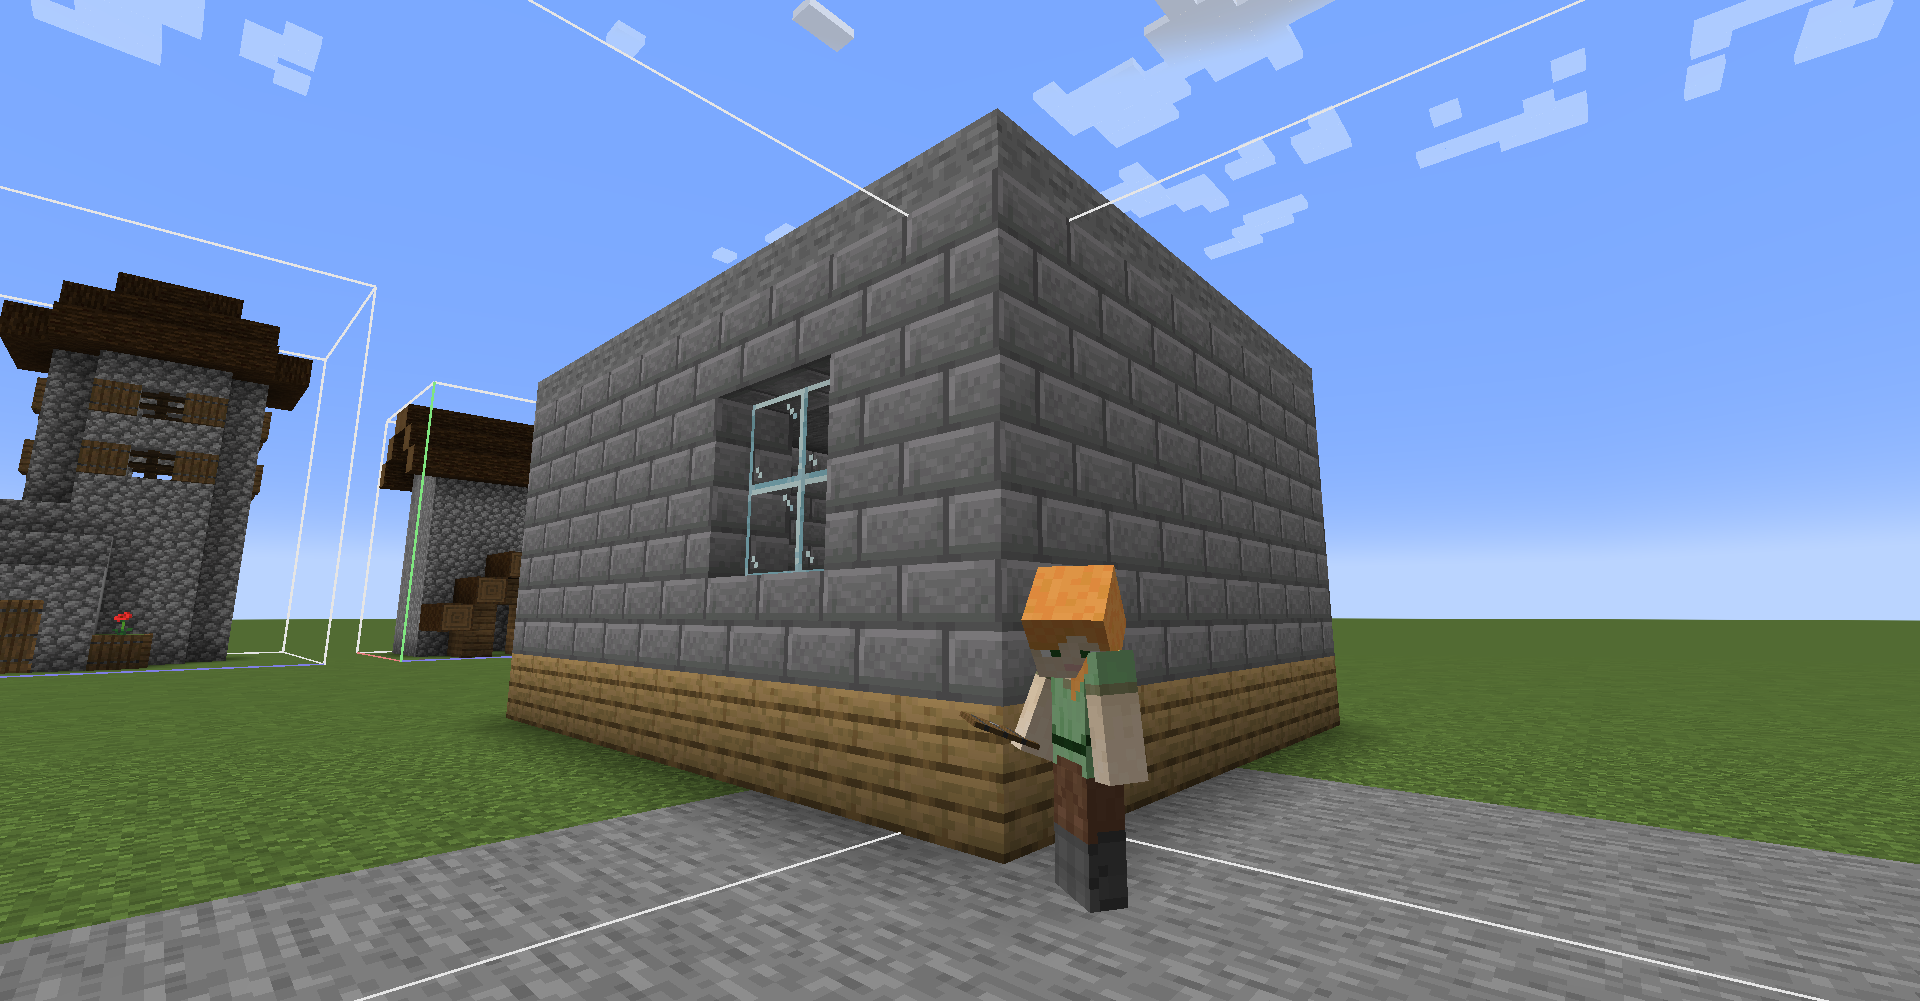
\includegraphics[width=0.7\textwidth]{fig/generate_example.png}
    \caption{構造物自動生成の生成結果}
    \label{fig:generate_example}
\end{figure}



\section{構造物自動生成のファインチューニング}
人間の作成した構造物を学習させる事によりより複雑な構造が生成できることが考えられたため、構造物自動生成のファインチューニングを行った。
ファインチューニング済みモデルを作成するまでの手順は学習データの作成とファインチューニングに分けて解説する。

\subsection{学習データの作成}
学習データを作成するための手順として、まず、大規模言語モデルに読み込ませたい建造物をクリエイティブモードで手作業で作成した。家、ビル、木、クリーパー (Minecraftの代表的なキャラクター) のオブジェ等図\ref{fig:train_structure}に示す計15種類の構造物を作成した。

\begin{figure}[H]
    \centering
    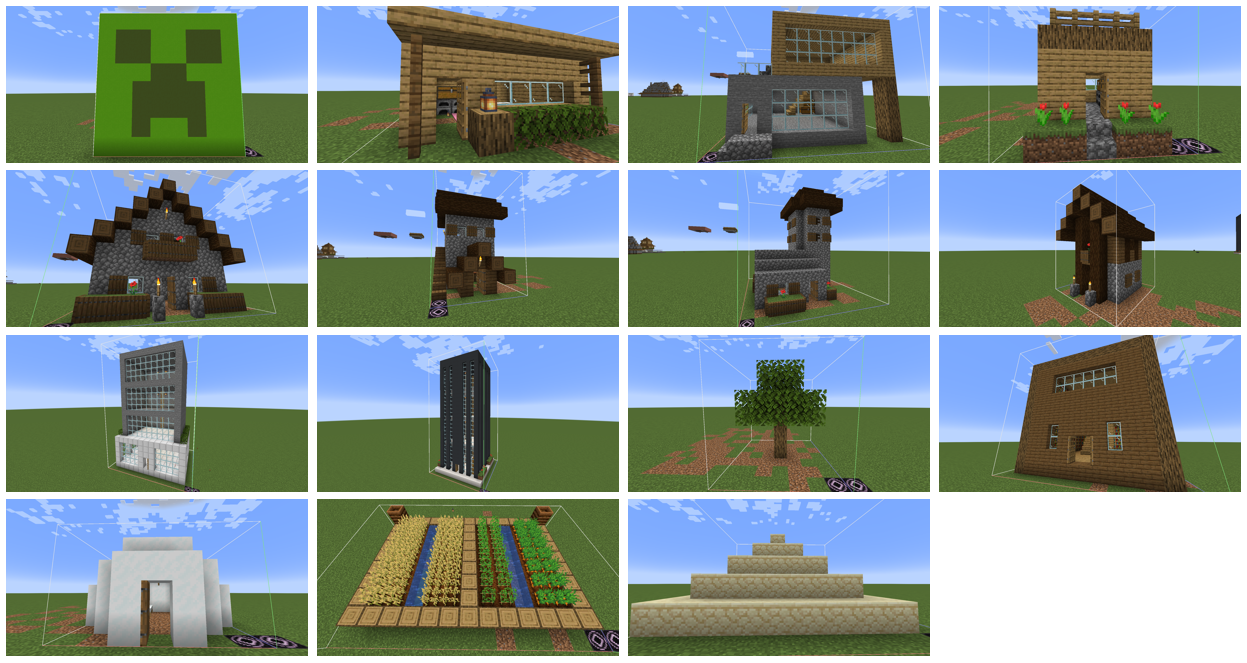
\includegraphics[width=0.95\textwidth]{fig/train_data.PNG}
    \caption{学習データの構造物}
    \label{fig:train_structure}
\end{figure}

次にストラクチャーブロックを用いて、手作業で作成した構造物をファイルに保存した。
ストラクチャーブロックとは範囲指定を行い、範囲内の構造物をNBTファイルとして保存したり、NBTファイルから構造物を読み出してMinecraft世界に出力することが可能なブロックである。
ストラクチャーブロックは図\ref{fig:structure_block}のような外観を有しており、通常の手段では入手できないものである。ストラクチャーブロックを入手するためにはゲームモードをクリエイティブモードの状態でチートを許可し以下のコマンドを実行すると入手可能である。
\begin{center}
    \textit{/give [player\_name] minecraft:structure\_block}
\end{center}

\begin{figure}[H]
    \centering
    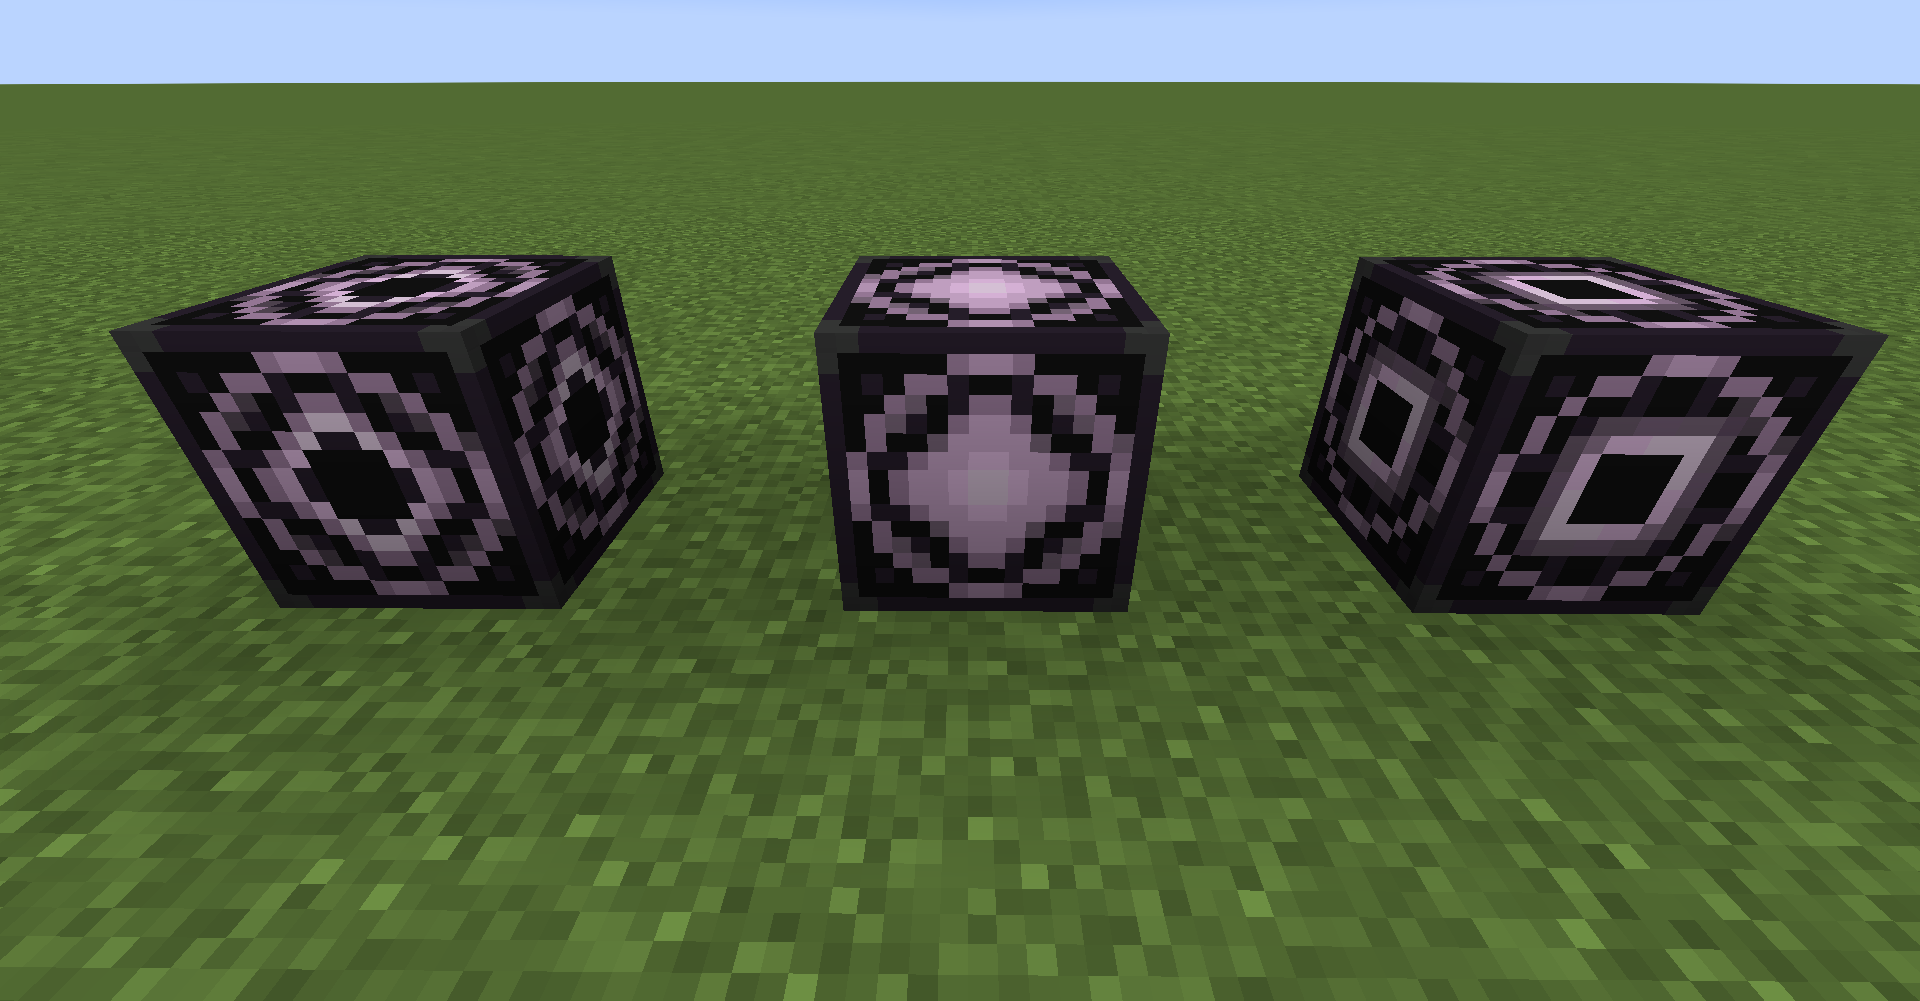
\includegraphics[width=0.7\textwidth]{fig/structure_block.png}
    \caption{ストラクチャーブロック}
    \label{fig:structure_block}
\end{figure}

構造物をファイルに保存した後は、データはNBTファイルというMinecraft固有のファイル形式であるためファイルの解析を行った。
NBTファイルの解析には外部ツールのPrismarine-NBT\cite{bib:prismarine-nbt}を用いた。
解析によって各座標に配置されたブロックの種類に関するデータのリスト得られたため各構造物に対して以下のアルゴリズムを適応しfillコマンドのリストを作成した。

\begin{enumerate}
    \item 重複を許した、2つのブロックの組み合わせを全て列挙する。
    \item 全ての2ブロックの組み合わせに対して、2ブロックを対角点とする直方体の範囲を作成する。
    \item 直方体の範囲内のブロックが、空気ブロック以外の同じブロックで満たされているものの中で最大の体積の直方体を抽出する。
    \item 抽出した最大の体積の直方体のデータをもとにfillコマンドを1つ作成する。fillコマンドを作成できたら抽出した直方体の範囲内のブロックを全て空気ブロックに置き換える。
    \item 全てのブロックが空気ブロックとなるまで3~4を繰り返す。
\end{enumerate}

最後に完成したfillコマンドのリストに、手動でアノテーション作業を行いfillコマンドで作成している部分の説明を加えた。

このような手順を踏むことで、構造物自動生成の学習データを作成した。
また、作成した学習データを分割し、装飾などの細部を少し変更したデータを作ることにより、合計19件の学習データを構築した。
完成した学習データ1件を、図\ref{fig:train_structure}左上のクリーパーのオブジェを例に次ページに示す。
\newpage
\noindent
user:

\noindent
\fbox{
    please make Creeper.
}

\noindent
assistant:

\noindent\fbox{
    \parbox{\textwidth}{
    This is a list of fill commands to create the face of the iconic Minecraft character ""Creeper"". \\
    The creeper is a typical Minecraft mob and is green. Therefore, we will create it using a green concrete block. \\
    We will create it by executing the /fill command in the following steps. \\
    \\
    1. Create the left eye with a 2x2 green concrete block. \\
    /fill \textasciitilde2 \textasciitilde5 \textasciitilde0 \textasciitilde3 \textasciitilde6 \textasciitilde0 minecraft:green\_concrete \\
    \\
    2. Create the right eye in the same way.\\
    /fill \textasciitilde6 \textasciitilde5 \textasciitilde0 \textasciitilde7 \textasciitilde6 \textasciitilde0 minecraft:green\_concrete\\
    \\
    3. Create a mouth with green concrete blocks. The creeper's mouth has a distinctive shape.\\
    /fill \textasciitilde3 \textasciitilde2 \textasciitilde0 \textasciitilde6 \textasciitilde3 \textasciitilde0 minecraft:green\_concrete\\
    /fill \textasciitilde4 \textasciitilde4 \textasciitilde0 \textasciitilde5 \textasciitilde4 \textasciitilde0 minecraft:green\_concrete\\
    /fill \textasciitilde3 \textasciitilde1 \textasciitilde0 \textasciitilde3 \textasciitilde1 \textasciitilde0 minecraft:green\_concrete\\
    /fill \textasciitilde6 \textasciitilde1 \textasciitilde0 \textasciitilde6 \textasciitilde1 \textasciitilde0 minecraft:green\_concrete\\
    \\
    4. Finally, create the contours of the face.\\
    /fill \textasciitilde1 \textasciitilde0 \textasciitilde0 \textasciitilde2 \textasciitilde4 \textasciitilde0 minecraft:lime\_concrete\\
    /fill \textasciitilde7 \textasciitilde0 \textasciitilde0 \textasciitilde8 \textasciitilde4 \textasciitilde0 minecraft:lime\_concrete\\
    /fill \textasciitilde1 \textasciitilde7 \textasciitilde0 \textasciitilde8 \textasciitilde7 \textasciitilde0 minecraft:lime\_concrete\\
    /fill \textasciitilde3 \textasciitilde0 \textasciitilde0 \textasciitilde6 \textasciitilde0 \textasciitilde0 minecraft:lime\_concrete\\
    /fill \textasciitilde4 \textasciitilde5 \textasciitilde0 \textasciitilde5 \textasciitilde6 \textasciitilde0 minecraft:lime\_concrete\\
    /fill \textasciitilde4 \textasciitilde1 \textasciitilde0 \textasciitilde5 \textasciitilde1 \textasciitilde0 minecraft:lime\_concrete\\
    /fill \textasciitilde1 \textasciitilde5 \textasciitilde0 \textasciitilde1 \textasciitilde6 \textasciitilde0 minecraft:lime\_concrete\\
    /fill \textasciitilde8 \textasciitilde5 \textasciitilde0 \textasciitilde8 \textasciitilde6 \textasciitilde0 minecraft:lime\_concrete\\
    /fill \textasciitilde3 \textasciitilde4 \textasciitilde0 \textasciitilde3 \textasciitilde4 \textasciitilde0 minecraft:lime\_concrete\\
    /fill \textasciitilde6 \textasciitilde4 \textasciitilde0 \textasciitilde6 \textasciitilde4 \textasciitilde0 minecraft:lime\_concrete\\
    }
}
\newpage

\subsection{ファインチューニング}
OpenAIドキュメントのFine-tuningページ\cite{bib:fine-tuning}を参考に学習データからjsonlファイルを作成しファインチューニングを行った。
ファインチューニング時の設定は以下の通りである。

\begin{table}[H]
    \caption{ファインチューニングの設定}\label{tab:finetuning}
    \centering
    \begin{tabular}{ll}
        \hline \hline
        モデル & gpt-3.5-turbo-1106 \\
        \hline
        学習データ & training\_data.jsonl \\
        \hline
        学習データ件数 & 19件 \\
        \hline
        エポック & 5 \\
        \hline
    \end{tabular}
\end{table}
\chapter{実験と結果}	
\thispagestyle{plain}   % chapterの直後に必ず指定

\section{タスクの提示や会話機能の動作テスト}\label{sec:gpt_res_test}
この節では\ref{sec:gpt_res}節で開発した{\mason}のサバイバルモードのプレイヤー向けの対話機能について、目標を設定し動作テストの結果を述べる.

今回は{\mason}に表\ref{tab:goal_and_action}の目標や使用できる行動を設定し、{\mason}との対話機能を使用した。

\begin{table}[H]
    \caption{実験1の設定}\label{tab:goal_and_action}
    \centering
    \begin{tabular}{ll}
        \hline \hline
        目標 & ダイヤモンドを集める. \\
        \hline
        許可した行動 & mine\_block \\
          & craft\_item \\
        \hline
    \end{tabular}
\end{table}

目標への最序盤での対話の結果を図\ref{fig:first_task}に示す。
図を見ると、{\mason}はプレイヤーが森バイオームに位置し何も装備していないことなどからゲームの序盤であることを推論し、Minecraftの最も基本的な資源の木を集めるべきであるとタスクを提示している。
また、``木を集める''というタスクは{\mason}も行うことが出来るタスクであるためこの作業を手伝うかの提案を行っている。

\begin{figure}[H]
    \centering
    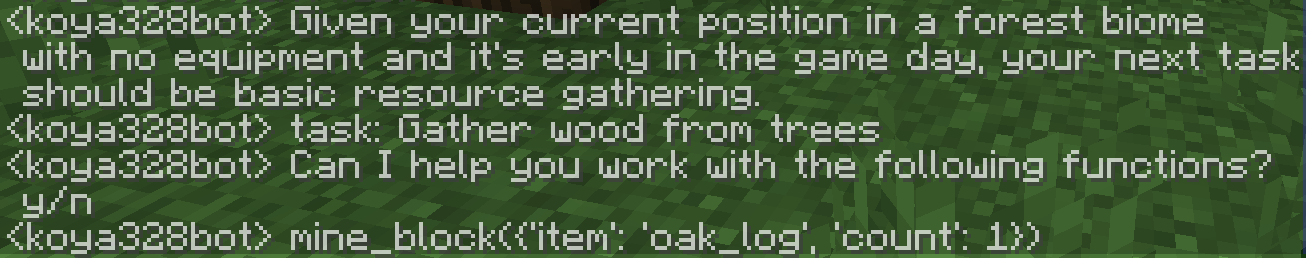
\includegraphics[width=0.95\textwidth]{fig/first_task.PNG}
    \caption{序盤のタスクの提示}
    \label{fig:first_task}
\end{figure}

木を切るタスクを手伝ってもらうために``y''で返答することで、図\ref{fig:task_help}のようにプレイヤーに提示したタスクを{\mason}も行うことが出来ている。
\begin{figure}[H]
    \centering
    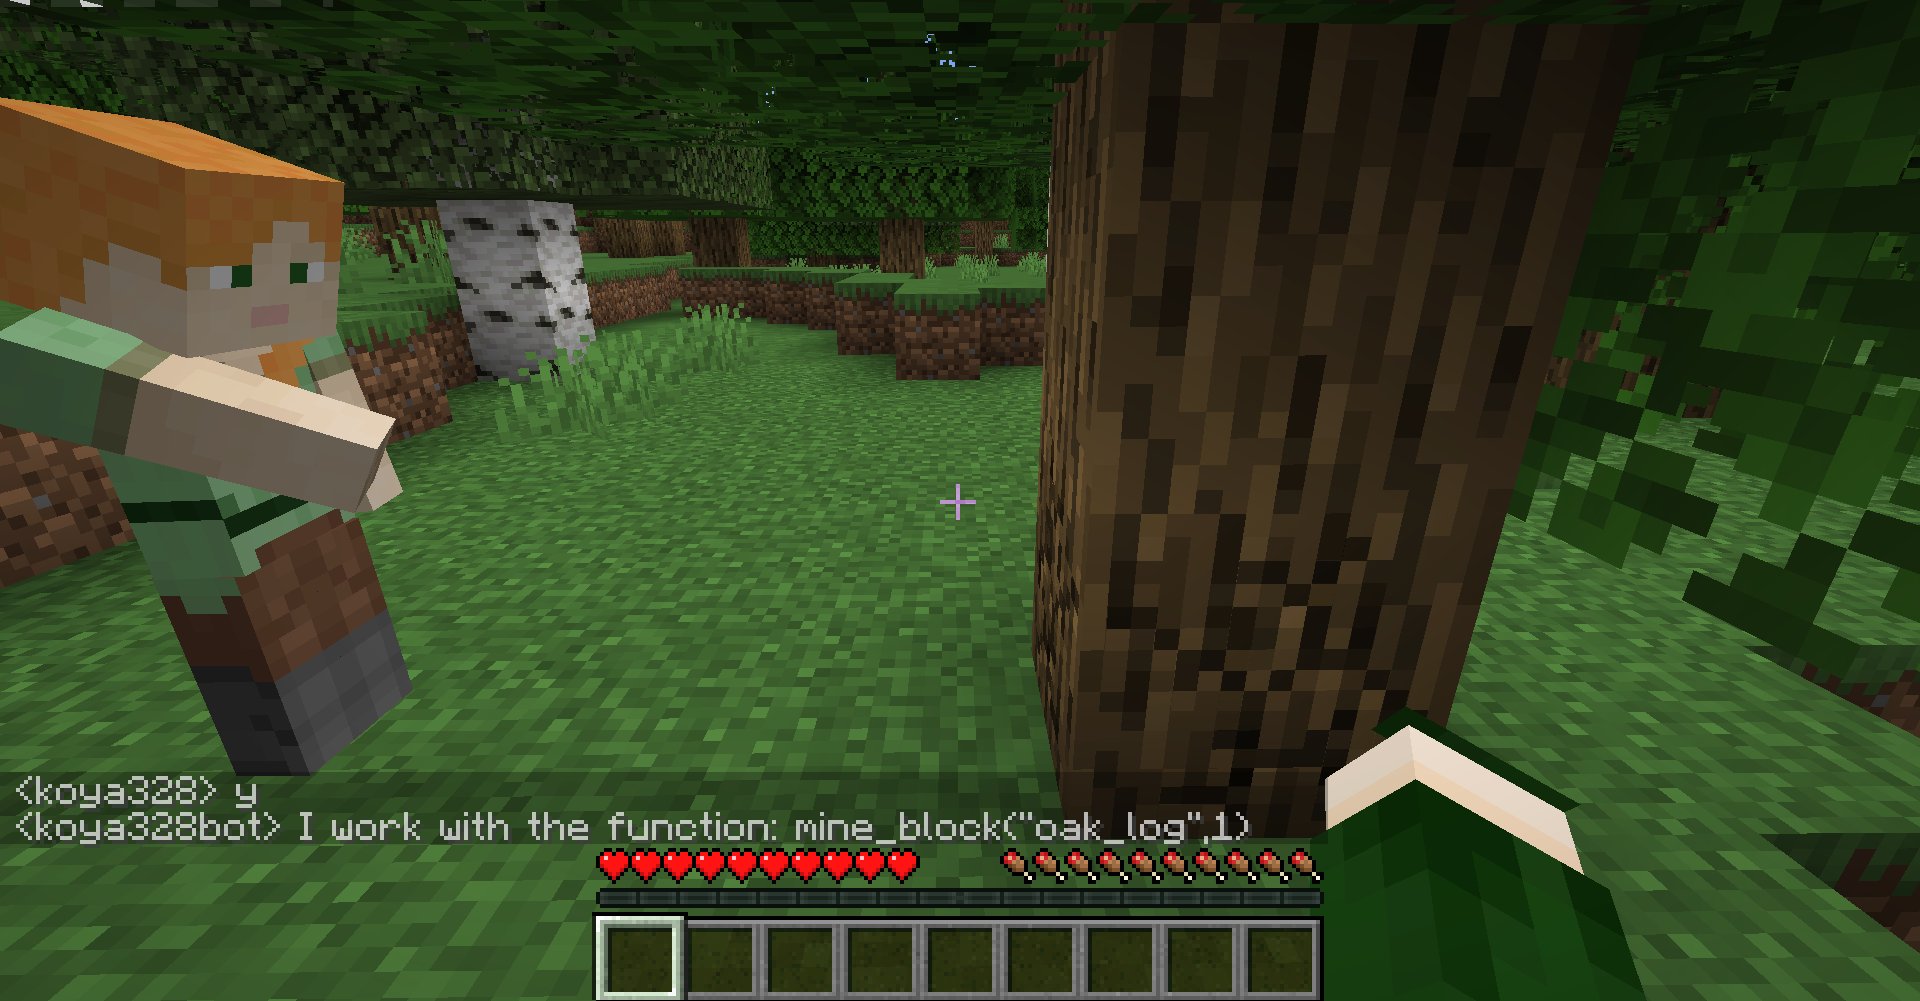
\includegraphics[width=0.95\textwidth]{fig/task_help.PNG}
    \caption{木を切る作業の支援}
    \label{fig:task_help}
\end{figure}

{\mason}はプレイヤーから話しかけられなくても定期的にタスクを提示することができ、木を切った後に図\ref{fig:wooden_pickaxe}のように木のピッケルを作るべきだというタスクを提示している。
木のピッケルの作り方がわからないプレイヤーが作り方を質問した場合、その質問に回答することが可能だった。
\begin{figure}[H]
    \centering
    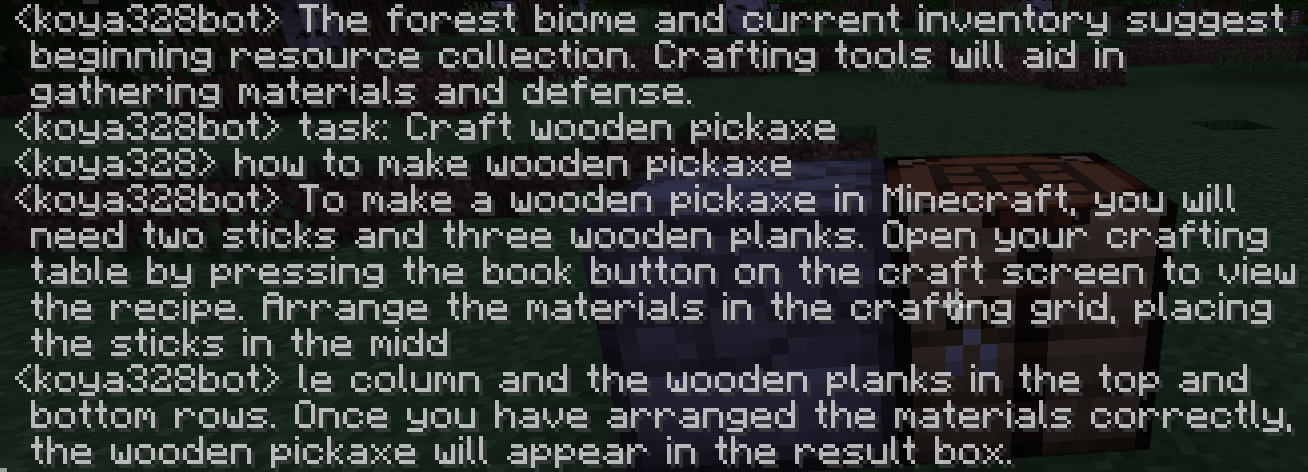
\includegraphics[width=0.95\textwidth]{fig/wooden_pickaxe.png}
    \caption{木を切る作業の支援}
    \label{fig:wooden_pickaxe}
\end{figure}

また、目標の達成とは関係ない質問 (図\ref{fig:diamond_question}はダイヤモンドを取得したあと何のアイテムを作ることが出来るかの質問)についても回答することが出来る。
\begin{figure}[H]
    \centering
    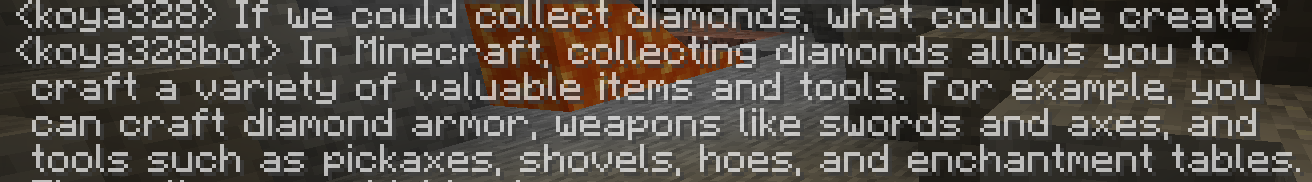
\includegraphics[width=0.95\textwidth]{fig/diamond_question.PNG}
    \caption{目標と関係ない質問をしたときの対話}
    \label{fig:diamond_question}
\end{figure}

目標の最終盤での対話の結果を図\ref{fig:final_task}に示す。
図を見ると、{\mason}はプレイヤー鉄のピッケルを持っていることからダイヤを採掘するタスクを提示出来ている。

\begin{figure}[H]
    \centering
    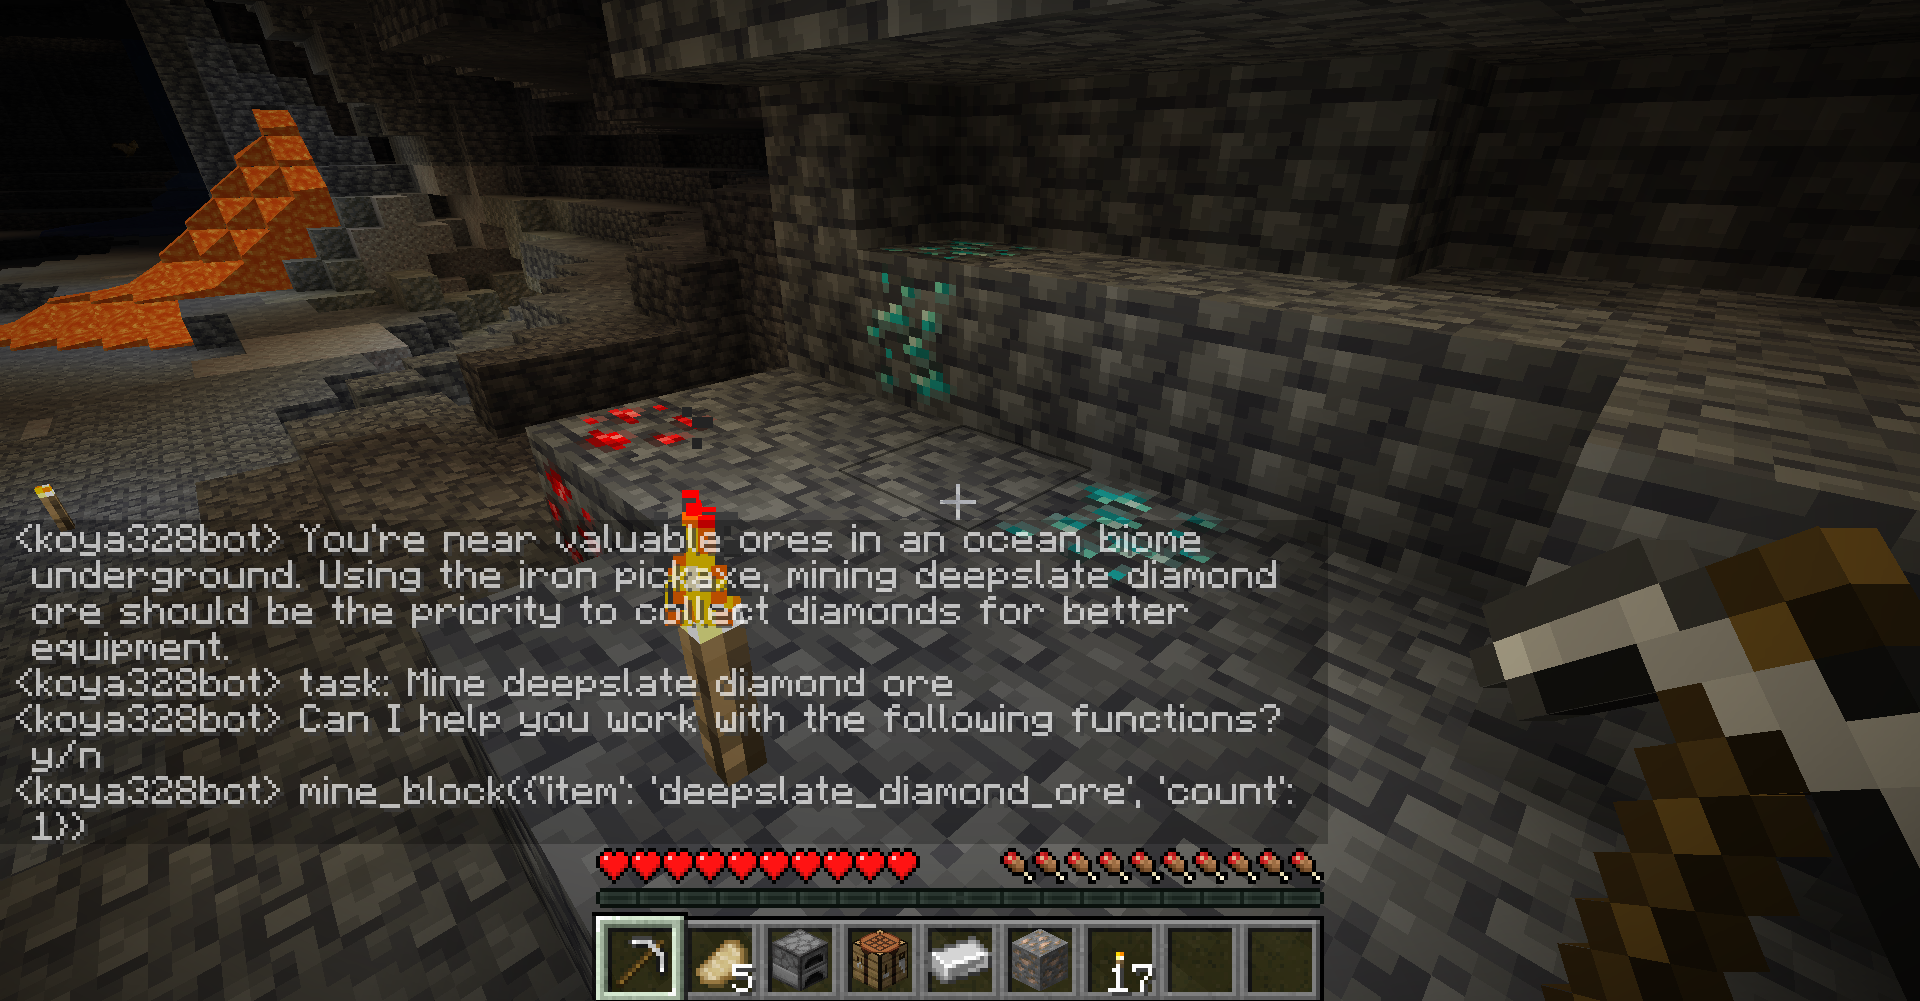
\includegraphics[width=0.95\textwidth]{fig/final_task.png}
    \caption{ダイヤモンド採掘の提示}
    \label{fig:final_task}
\end{figure}

\section{構造物自動生成の実験}\label{sec:build_mode_generate}
この節では,\ref{sec:build_mode}節にて解説したクリエイティブモード向け構造物自動生成機能がどのような構造物を生成可能であるかを,モデルやプロンプトの設定を踏まえて紹介する.

\subsection{実験1}\label{sec:ex1}
実験1では,{\mason}の自動生成機能において,詳細度の異なる2つのプロンプトをそれぞれ送信し,出力結果の比較を行った.今回の実験の設定内容は表\ref{tab:setting1}に記す.
今回のテストケースとして駅の構造を生成した.
なお,大規模言語モデルによる出力結果は一定ではないため,表\ref{tab:setting1}のとおり,それぞれのプロンプトを3度送信した.
その中から,それぞれ最も優れた結果を図\ref{fig:station1}に示す.
\begin{table}[H]
    \caption{実験1の設定}\label{tab:setting1}
    \centering
    \begin{tabular}{ll}
        \hline \hline
        モデル & gpt-3.5-turbo \\
        \hline
        左図プロンプト & train station \\
        \hline
        右図プロンプト & Build a train station.I want the tracks to use rails. \\
          & And build the platform well. \\
        \hline
        試行回数 & 3回 \\
        \hline
    \end{tabular}
\end{table}

\begin{figure}[H]
    \centering
    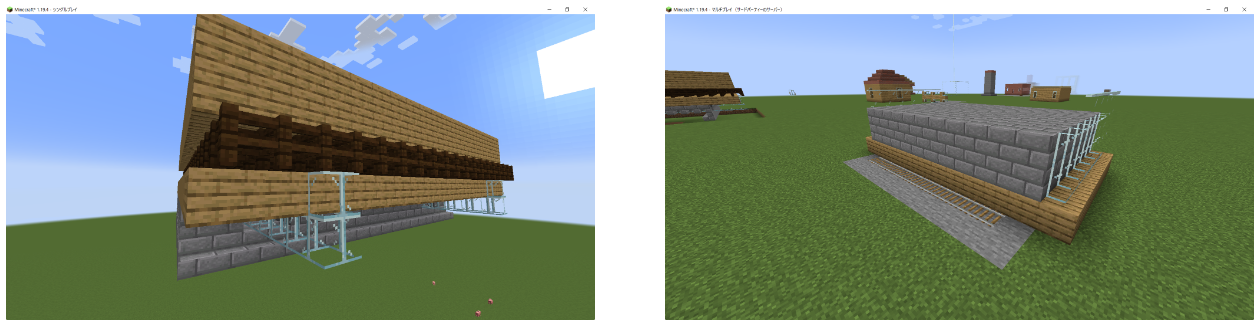
\includegraphics[width=0.95\textwidth]{fig/train_station1.PNG}
    \caption{実験1の生成結果}
    \label{fig:station1}
\end{figure}

図\ref{fig:station1}右図の出力結果を見ると駅の外装のような構造物を作成していることが示唆される.
しかし,左図構造物生成時のログを参照すると,下部の石レンガはプラットフォーム,上部の板材,ダークオークのフェンス,ガラスパネルはチケットカウンター,ベンチ,標識であると記載されているため,この出力結果は駅の外装ではなくモデルがあまり駅のプラットフォームについて理解せず生成したものであると言える.
右図では,ログを参照したところ板材と石レンガでプラットフォームを作り,それに沿うようにレールを敷いていると記載されているため,プロンプトによって出力改善されたことが分かる.

\subsection{実験2}\label{sec:ex2}
実験2では,{\mason}の自動生成機能において,詳細度の異なる2つのプロンプトをそれぞれ送信し,出力結果の比較を行った.今回の実験の設定内容は表\ref{tab:setting2}に記す.
実験1と同様に今回のテストケースとして駅の構造を生成した.
なお,大規模言語モデルによる出力結果は一定ではないため,表\ref{tab:setting2}のとおり,それぞれのプロンプトを3度送信した.
その中から,それぞれ最も優れた結果を図\ref{fig:station2}に示す.
\begin{table}[H]
    \caption{実験2の設定}\label{tab:setting2}
    \centering
    \begin{tabular}{ll}
        \hline \hline
        モデル & gpt-4 \\
        \hline
        左図プロンプト & train station \\
        \hline
        右図プロンプト & Build a train station.I want the tracks to use rails. \\
          & And build the platform well. \\
        \hline
        試行回数 & 3回 \\
        \hline
    \end{tabular}
\end{table}

\begin{figure}[H]
    \centering
    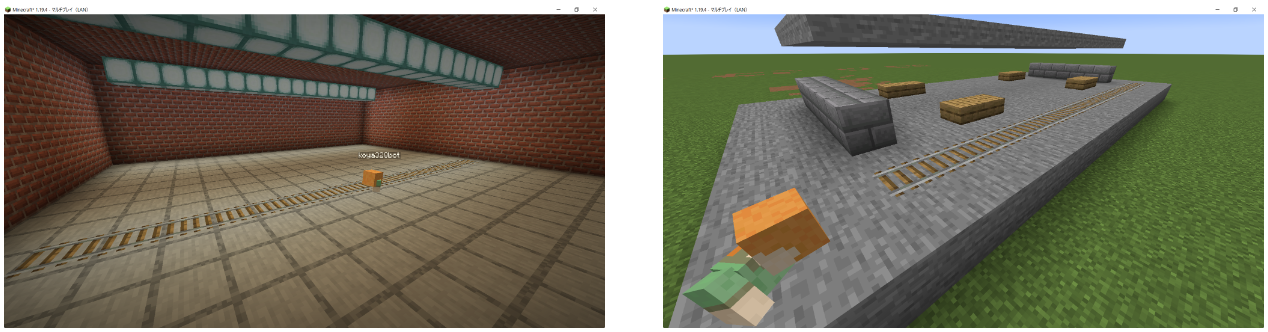
\includegraphics[width=0.95\textwidth]{fig/train_station2.PNG}
    \caption{実験2の生成結果}
    \label{fig:station2}
\end{figure}

\subsection{実験3}\label{sec:ex3}
実験3では,{\mason}の自動生成機能において,プロンプトによる構造物の生成を行い,その後追加のプロンプトを送信し,出力結果がどのように変化するかを検証した.今回の実験の設定内容は表\ref{tab:setting3}に記す.
今回のテストケースとしてまず家を作成するプロンプト(表\ref{tab:setting3}プロンプト1)を送信し,その後窓を追加するプロンプト(表\ref{tab:setting3}プロンプト2)を送信した.
なお,大規模言語モデルによる出力結果は一定ではないため,表\ref{tab:setting3}のとおり,プロンプトを3度送信し,その中から,最も優れた結果を図\ref{fig:add_window}に示す.

\begin{table}[H]
    \caption{実験3の設定}\label{tab:setting3}
    \centering
    \begin{tabular}{ll}
        \hline \hline
        モデル & gpt-4-1106-preview (GPT-4-Turbo) \\
        \hline
        プロンプト1 & please make house. \\
        \hline
        プロンプト2 & please add window. \\
        \hline
        試行回数 & 3回 \\
        \hline
    \end{tabular}
\end{table}

\begin{figure}[H]
    \centering
    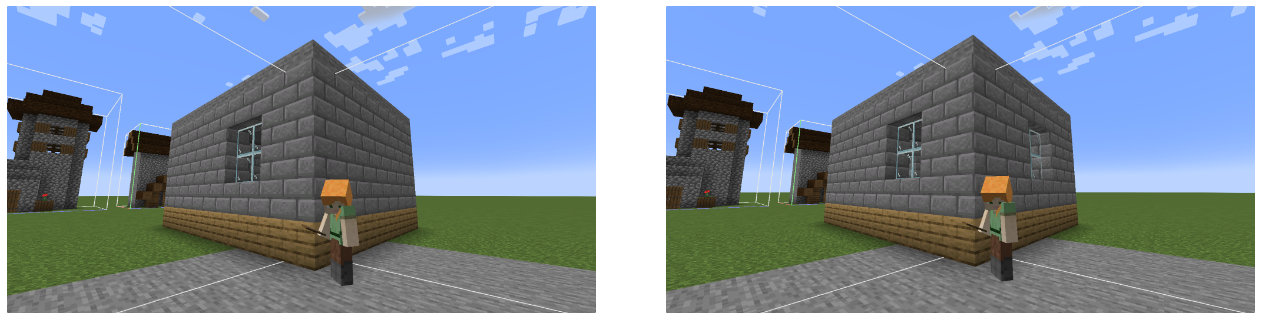
\includegraphics[width=0.95\textwidth]{fig/add_window.PNG}
    \caption{実験3の生成結果}
    \label{fig:add_window}
\end{figure}

\subsection{実験4}\label{sec:ex4}
実験4では,{\mason}の自動生成機能において,プロンプトによる構造物の生成を行い,その後追加のプロンプトを送信し,出力結果がどのように変化するかを検証した.今回の実験の設定内容は表\ref{tab:setting4}に記す.
実験3と同様にテストケースとしてまず家を作成するプロンプト(表\ref{tab:setting4}プロンプト1)を送信し,その後窓を追加するプロンプト(表\ref{tab:setting4}プロンプト2)を送信した.
なお,大規模言語モデルによる出力結果は一定ではないため,表\ref{tab:setting4}のとおり,プロンプトを3度送信し,その中から,最も優れた結果を図\ref{fig:add_window2}に示す.

\begin{table}[H]
    \caption{実験4の設定}\label{tab:setting4}
    \centering
    \begin{tabular}{ll}
        \hline \hline
        モデル & gpt-3.5-turbo-1106ファインチューニング済みモデル \\
        \hline
        プロンプト1 & please make house. \\
        \hline
        プロンプト2 & please add window. \\
        \hline
        試行回数 & 3回 \\
        \hline
    \end{tabular}
\end{table}

\begin{figure}[H]
    \centering
    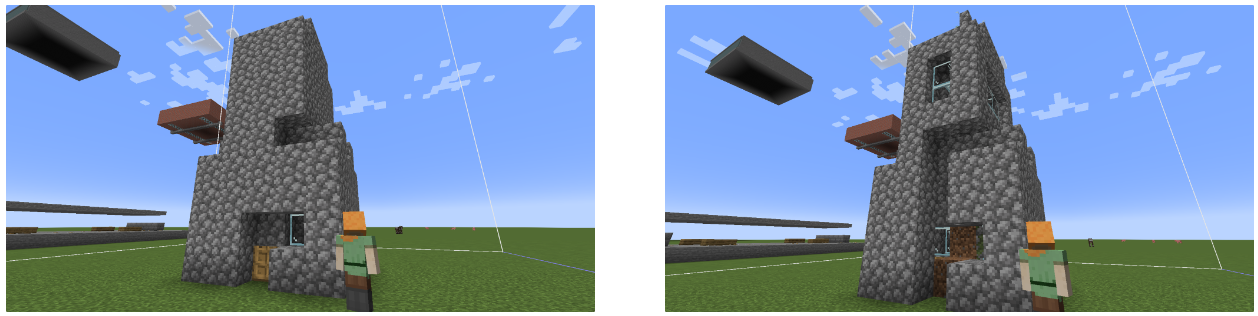
\includegraphics[width=0.95\textwidth]{fig/add_window2.PNG}
    \caption{実験3の生成結果}
    \label{fig:add_window2}
\end{figure}

\section{アンケートの実施と結果}\label{sec:survey_result}
botの有用性を検証するためbotのデモとアンケートを実施した.
デモ・アンケートは2023年10月16日に開催された,公立はこだて未来大学オープンラボの,イアンフランク研ブースにて行われ,計16人の学生がデモを行いアンケートに回答した.
デモではbotとの会話を始めに体験していただき,その後,ビルドモードを体験するように促した.

デモを行った後のアンケートの結果の一例について表\ref{tab:answer1},表\ref{tab:answer2}に示す.

``このbotを使うことで新しい建築のアイデアやインスピレーションを得ることができましたか?''という質問について,``そう思う''を4,``どちらかというとそう思う''を3,``どちらかというとそう思わない''を2,``そう思わない''を1として平均を計算した結果,3.2 となった.
表\ref{tab:answer1}の結果では肯定的な意見が得られているものの,表\ref{tab:answer2}の結果より平均が低いことや\ref{sec:build_mode_generate}節の生成結果から考察するとビルドモードは改善の必要があると考えられる.
\begin{table}[H]
    \centering
    \caption{このbotを使うことで新しい建築のアイデアやインスピレーションを得ることができましたか?}
    \label{tab:answer1}
    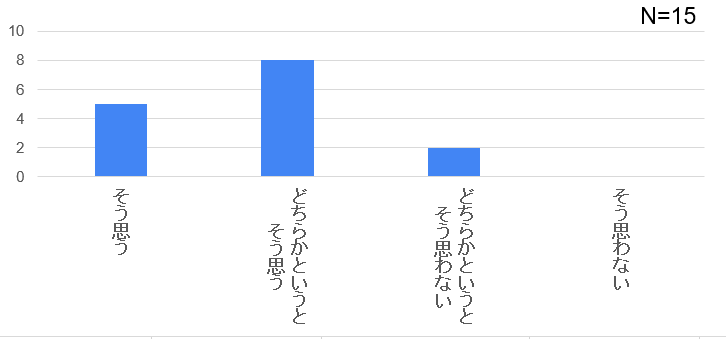
\includegraphics[width=0.7\textwidth]{fig/tab2.png}
\end{table}

また,``このbotを使うことで大規模言語モデル(ChatGPTなど)の使い方を新しく学ぶことができましたか?''の質問については同様の方法で平均を求めた結果,3.47となった.

\begin{table}[H]
    \centering
    \caption{このbotを使うことで大規模言語モデル(ChatGPTなど)の使い方を新しく学ぶことができましたか?}
    \label{tab:answer2}
    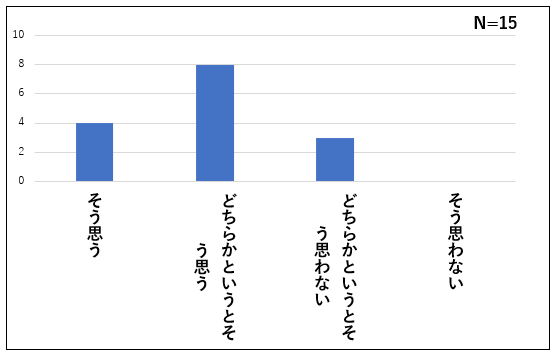
\includegraphics[width=0.7\textwidth]{fig/tab3.png}
\end{table}

そう思う~そう思わないの4段階の同じ指標で回答してもらった結果,表\ref{tab:answer2}の結果のみ平均3.47と高かったことから,botによって大規模言語モデルの新しい使い方を学べたことが示唆された.





\chapter{考察}
\thispagestyle{plain}   % chapterの直後に必ず指定

この章では5章での実験やテストの結果を考察し,最終的に本研究の目的である,人間とAIの協調の限界・可能性について考察する.

\section{タスクの提示や会話機能の考察}\label{sec:gpt_res_investigation}
この節では,先述の\ref{sec:gpt_res_test}節の動作テストについて考察する.
\ref{sec:gpt_res_test}節では,{\mason}とプレイヤーが対話を行い,{\mason}は現在の進行度に合わせたタスクの提示や作業支援,質問への回答が可能であることを確認できた.

このことから,大規模言語モデルに対して現在の状態を正しく伝えることが可能であれば,次のタスクを提示できることが示唆された.
また,目標に寛解のない事柄などに関しても回答できる能力を有していることが示唆された.

LLMがプレイヤーが次に行うべきステップを提案し,ピッケルの作り方などプレイヤー未知のタスクについて指導できることは,ゲームを通じた学習サポートツールとしての応用も可能であることを示唆している.
このようなサポートツールとしての使い方であれば,特にコミュニケーションスキルや問題解決スキルを向上させることが可能であると示唆される.
また,プレイヤーがbotとの対話の方法のみを知ることができれば,人間の教育者を必要とせずAIとの対話によって自律的に学習ができる未来が考えられる.

しかし,稀に次に提示するタスクが適切ではないことや,質問に対する回答が間違っている結果が確認された.
大規模言語モデルは出力が一定ではなく,出力される結果が必ずしもあっているとは限らないという特徴があり,この結果もそのデメリットの影響を受けている考えられる.
したがって現状では,{\mason}が誤った情報を回答しないように,RAGの機能で知識に基づいた回答を行うようにすることや,{\mason}を扱うときも他の大規模言語モデルと同様に,結果を鵜呑みにせず事実確認を徹底する必要があると考えられる.

\section{構造物生成の考察}\label{sec:generate_investigation}
この節では,先述の\ref{sec:build_mode_generate}節及び各小節における実験結果を考察する.
\ref{sec:build_mode_generate}節では,ビルドモードによる構造物の生成が行われたが,その結果から,いくつかの特筆すべき傾向が存在した.

\ref{sec:ex4}節の実験では,ファインチューニングされたgpt-3.5-turboモデルを使用し,その結果から複雑な構造物を生成する能力が向上したことが示唆された.
しかし,その一方で問題も生じており,その一つが建物内部の構造を埋めてしまう現象である.
これは,gpt-3.5-turboが内部構造の設計を適切に行えない,という可能性を指摘している.
また,ファインチューニング前の同モデルで駅を生成した\ref{sec:ex1}節の実験でも同様の問題が見られ,チケットカウンター,ベンチ,標識等の配置が適切でない,という結果が得られている.

一方で,モデルが更新されたgpt-4やgpt-4-turboを用いた実験,\ref{sec:ex2}節および\ref{sec:ex3}節では,この問題は見られなかった.
ここでは,それらのモデルが内部空間を適切に設計し,窓を正しい位置に配置する能力を示していた.
これは,これらのモデルが空間把握能力を著しく向上させていると考えられる.

これらの結果から,gpt-3.5-turboは空間把握能力が限定的であり,このモデルをさらにファインチューニングしても,人間と同様に複雑な構造を構築する能力を獲得するのは難しいと推測することができる.
しかし,後継のgpt-4やgpt-4-turboを用いれば,より複雑な構造物の生成が可能になると期待される.
これらのファインチューニングが実現すれば,より高度な建造物生成が可能となり,人間により強い建築のインスピレーションなどを与える可能性があると考えられる.

\section{アンケートの考察}\label{sec:survey_investigation}
この節では,先述の\ref{sec:survey_result}節及び各小節における実験結果を考察する.
アンケートの結果はすべての回答の平均が3を超えていたことから,肯定的な意見を得ることができた.
その中でも,そう思う,どちらかというとそう思う,どちらかというとそう思わない,そう思わないの4段階の同じ指標で回答してもらった結果,表\ref{tab:answer2}の結果のみ平均3.47と高かったことから,botによって大規模言語モデルの新しい使い方を学べたことが示唆された.

\section{考察}
この節では,\ref{sec:gpt_res_investigation}節~\ref{sec:survey_investigation}節の考察をもとに本研究の目的である,人間とAIの協調の限界・可能性について考察する.

\ref{sec:gpt_res_investigation}節~\ref{sec:survey_investigation}節の考察から,
AIとの協調により,学習効果や創造的なインスピレーションを得られること目的として,botを作成した結果,タスクの提示や支援,構造物生成などテストレベルでの興味深い結果を得られることが判明した.
しかし,現状では提示されたタスクが必ずしも合っているとは限らないことや複雑な構造物を生成できないことなどの問題があり,実用段階に至るにはまだいくつかの発展が必要であるという課題が示唆された.

しかし近年の大規模言語モデルの発展は著しく,現状のgpt-4-turboでは空間把握能力を有していることが示唆されたため,gpt-4-turboなどのモデルがファインチューニング可能になることや,より高精度なモデルが登場することによって,
将来的にはコミュニケーションスキルや問題解決スキル,創造的なインスピレーションをAIから得られる可能性が考えられる.
%他の環境への適応
\chapter{まとめ・展望}	% TODO: 章題を記入.題は任意.
\thispagestyle{plain}   % chapterの直後に必ず指定

%TODO: 章の内容を記入.以下はサンプル.
\section{まとめ}
本研究は,人間とAIの協力・協調関係を築くことを目的とし,Minecraftの中で人間との対話や,作業の支援を行うBOTの作成を行った.
また,BOTのデモを行った後のアンケートの結果から,LLMの新たな使い方を学べたことが示唆された.

\section{展望}
BOTのビルドモードは,これまで想像力を必要としていたものを,プロンプトによって瞬時に創造できるようになる可能性を示唆しているが現在の機能は初期の段階であり,今後の予定としては,プロンプトの改善によってより複雑な構造物を生成し,より強いインスピレーションを得られるようにする必要があると考えられる.
% 以下必要に応じてchapterX.texを作成してinput文を記入

% TODO: 謝辞
\pagestyle{plain}
\chapter*{謝辞}
% TODO: 謝辞を以下に記入

本研究において, 数々のご指導を賜りましたIan Frank教授, {\mason}のテスト環境を提供してくださったFUN Minecraft Serverの運営の皆様に深くお礼申し上げます。


% TODO: 発表等実績
\chapter*{発表・採録実績}

% TODO: 発表・採録実績(確定分も含む)を以下の例のように記入

\subsection*{発表等}
\begin{enumerate}
\renewcommand{\labelenumi}{[\arabic{enumi}]}
    \item 発表その1
    \item 発表その2
    \item 発表予定(発表予定年月)
\end{enumerate}

\subsection*{学術論文,国際会議等(査読付き)}
\begin{enumerate}
\renewcommand{\labelenumi}{[\arabic{enumi}]}
    \item 論文その1
    \item 国際会議その1
    \item 採録決定論文(採録予定年月)
\end{enumerate}


% TODO: 参考文献
\begin{thebibliography}{99}
%chapter1
\bibitem{bib:chess}
    J. McCarthy. (2007) 
    ``What is Artificial Intelligence?'', 
    \url{http://www-formal.stanford.edu/jmc/whatisai/whatisai.html} (Accessed 2023/10/31).
\bibitem{bib:AplpaGo}
    D. Silver, A. Huang, C. J. Maddison et al. (2016) 
    Mastering the game of Go with deep neural networks and tree search, 
    Nature volume 529, pp.484-489.
\bibitem{bibAlphaStar}
    O. Vinyals, I. Babuschkin, W. M. Czarnecki et al. (2019) 
    Grandmaster level in StarCraft II using multi-agent reinforcement learning, 
    Nature volume 575, pp.350-354.
\bibitem{bib:maia}
    R. McIlroy-Young, S. Sen, J. Kleinberg, A. Anderson. (2020) 
    Aligning Superhuman AI with Human Behavior: Chess as a Model System,
    KDD '20: Proceedings of the 26th ACM SIGKDD International Conference on Knowledge Discovery \& Data Mining, pp 1677-1687.
\bibitem{bib:craft_assist}
    J. Gray, K. Srinet, Y. Jernite et al. (2019) 
    Craftassist: A framework for dialogue-enabled interactive agents,
    arXiv preprint arXiv:1907.08584.
\bibitem{bib:chatgpt}
    OpenAI. (2024)
    ``ChatGPT'',
    \url{https://chat.openai.com/auth/login} (Accessed 2024/01/11).
\bibitem{bib:chatgpt_news}
    Gigazine. (2023)
    ``ChatGPTが「月間1億ユーザー」をわずか2カ月で達成し史上最も急速に成長していることが報告される'',
    \url{https://gigazine.net/news/20230203-chatgpt-fastest-growing/} (Accessed 2024/01/11).
\bibitem{bib:citegpt}
    B. P. Teja. (2023)
    ``SiteGPT - Make AI your expert customer support agent'',
    \url{https://sitegpt.ai/} (Accessed 2024/01/11).
\bibitem{bib:slidegpt}
    SlidesGPT. (2023)
    ``SlidesGPT - AI PowerPoint Presentations, Powered by ChatGPT API'',
    \url{https://slidesgpt.com/} (Accessed 2024/01/11).
\bibitem{bib:Minecraft}
    Mojang Studios. (2023)
    ``Minecraft'', 
    \url{https://www.minecraft.net/ja-jp} (Accessed 2023/11/12).
\bibitem{bib:minecraft_news}
    Yahooニュース. (2023)
    ``『マインクラフト(Minecraft)』の累計売り上げが3億本を突破!史上最も売れたインディーゲーム,不動の地位を築く'',
    \url{https://news.yahoo.co.jp/articles/81edc817187b79350186eed8b5219f6be51a3ac7} (Accessed 2023/11/12).
%chapter2
\bibitem{bib:minecraft_creative tool}
	M. Cipollone, C. C. Schifter, R. A. Moffat. (2014) 
    Minecraft as a Creative Tool: A Case Study, 
    International Journal of Game-Based Learning 4(2), pp.1-14.
\bibitem{bib:arlpcg}
	L. Gisslén, A. Eakins, C. Gordillo et al. (2021)
    Adversarial Reinforcement Learning for Procedural Content Generation,
    2021 IEEE Conference on Games (CoG), pp1-8.
\bibitem{bib:gancraft}
	Z. Hao, A. Mallya, S. Belongie, M. Y. Liu. (2021) 
    GANcraft: Unsupervised 3D Neural Rendering of Minecraft Worlds, 
    Proceedings of the IEEE/CVF International Conference on Computer Vision, pp.14072-14082.
\bibitem{bib:voyager}
    G. Wang, Y. Xie, Y. Jiang et al. (2023)
    Voyager: An Open-Ended Embodied Agent with Large Language Models, 
    arXiv preprint arXiv: Arxiv-2305.16291.
%chapter3
\bibitem{bib:curseforge}
    Overwolf. (2024) 
    ``CurseForge - Minecraft Mods \& Modpacks'',
    \url{https://www.curseforge.com/minecraft} (Accessed 2024/01/09).
\bibitem{bib:eula}
    Mojang Studios. (2023)
    ``Minecraft End(er)-User License Agreement (``EULA'')'',
    \url{https://www.minecraft.net/en-us/eula} (Accessed 2024/01/09).
\bibitem{bib:minecraft_edu}
    Mojang Studios, (2023)
    ``Minecraft Education'', 
    \url{https://education.minecraft.net/ja-jp} (Accessed 2024/01/08).
\bibitem{bib:fun_minecraft_server}
    S. Kabashima, K. Matsuda, R. Yamamoto, I. Frank. (2023) 
    Building a Better World: Lessons from Setting up, Maintaining and Developing a University Minecraft Server, 
    JSET Autumn Conference 2023 collection papers. pp.597-598.
\bibitem{bib:cambridge_minecraft_server}
    University of Cambridge. (2020)
    ``Minecraft Cambridge: The platform for an online community''
    \url{https://www.cst.cam.ac.uk/undergraduate-creates-platform-virtual-community} (Accessed 2024/01/09).
\bibitem{bib:texas_minecraft_server}
    The University of Texas at Dallas, (2022)
    ``Creating Our University’s Official Minecraft Server | UT Dallas Esports''
    \url{https://esports.utdallas.edu/2022/03/14/creating-university-minecraft-server/} (Accessed 2024/01/09).
\bibitem{bib:tducraft}
    東京電機大学 TDUCraft有志. (2020)
    ``TDUCraft - マインクラフトサーバー''
    \url{https://www.tducraft.com/} (Accessed 2024/01/09).
\bibitem{bib:fun_minecraft_server_research}
    K. Kudo, K. Matsuda, I. Frank, D. K. Bagenda. (2023)
    Research and Education Through a Minecraft Testbed: Character, Bots and ChatGPT,
    JSET Autumn Conference 2023 collection papers. pp.595-596.
\bibitem{bib:fun_minecraft_server_research2}
    S. Kabashima, K. Sakabe, I. Frank, D. K. Bagenda. (2023) 
    Fostering Virtual Communities: The Impact of Analytics Tools in a University Minecraft Server, 
    JSET Spring Conference 2024 collection papers. (to appear)
%chapter4
\bibitem{bib:Mineflayer}
    PrismarineJS. (2024) 
    ``Github - PrismarineJS/mineflayer'', 
    \url{https://github.com/PrismarineJS/mineflayer} (Accessed 2024/01/09).
\bibitem{bib:few-shot}
    T. Brown, B. Mann, N. Ryder et al. (2020) 
    Language Models are Few-Shot Learners, 
    Advances in neural information processing systems volume 33, pp.1877-1901.
\bibitem{bib:rag}
    P. Lewis, E. Perez, A. Piktus et al. (2020) 
    Retrieval-Augmented Generation for Knowledge-Intensive NLP Tasks, 
    NeurIPS.
\bibitem{bib:function_calling}
    OpenAI. (2024)
    ``Function calling -Documentation'',
    \url{https://platform.openai.com/docs/guides/function-calling} (Accessed 2024/01/09).
\bibitem{bib:prismarine-nbt}
    PrismarineJS. (2023) 
    ``Github - PrismarineJS/prismarine-nbt: An NBT parser for node-minecraft-protocol'', 
    \url{https://github.com/PrismarineJS/prismarine-nbt} (Accessed 2024/01/09).
\bibitem{bib:fine-tuning}
    OpenAI. (2024) 
    ``OpenAI API - Fine-tuning'', 
    \url{https://platform.openai.com/docs/guides/fine-tuning} (Accessed 2024/01/09).
%chapter5

%chapter6

%chapter7





\end{thebibliography}


% 図表一覧等自動生成
\listoffigures
\thispagestyle{plain}
\listoftables
\thispagestyle{plain}


\end{document}
